% Document class (keine Änderungen hier)
\documentclass[a4paper,oneside,bibliography=totoc]{scrartcl}

% Encoding und Sprachen
\usepackage[utf8]{inputenc}
\usepackage[english]{babel}

% Mathematische Pakete
\usepackage{amsmath}
\usepackage{amssymb}
\usepackage{amsfonts}
\usepackage{amsthm} % Hier richtig platziert

% Grafik und Layout
\usepackage{graphicx}
\usepackage{tabularx}
\usepackage{booktabs}
\usepackage{multicol}
\usepackage{subcaption}

% Sonstige nützliche Pakete
\usepackage{latexsym}
\usepackage{csquotes}
\usepackage{cancel}
\usepackage{accents}
\usepackage{makeidx}
\usepackage{listings}
\usepackage{algorithm}
\usepackage{algorithmic}
\renewcommand{\algorithmiccomment}[1]{\hfill\textit{// #1}}

% Hyperlinks und Farben
\usepackage[hidelinks]{hyperref} % `hidelinks` vermeidet sichtbare Link-Kästen
\usepackage[usenames,dvipsnames]{xcolor} % Farbe für Hyperlinks
\hypersetup{
    colorlinks=true,
    citecolor=Green,  % Zitatfarben auf Grün gesetzt
}

% Literaturstil
\usepackage{natbib}
\bibliographystyle{chicagoa}
\setcitestyle{authoryear,round,semicolon,aysep={},yysep={,}}
\let\cite\citep

% Definitionen, Propositionen und Bemerkungen
\newtheorem{defn}{Definition}[section] % Definition-Umgebung, [section] für Nummerierung nach Abschnitten
\newtheorem{prop}{Proposition}[section]
\newtheorem{rem}{Remark}[section]
\newtheorem{Satz}{Theorem}[section]
\newtheorem{ex}{Example}[section]
\begin{document}

\subject{Report - Machine Learning (HWS 2024)} % change to appropriate type
\title{Assignment 2: Logistic Regression}
\author{Arne Huckemann (ahuckema), Elise Wolf (eliwolf)}
\date{\today}
\maketitle


\begin{abstract}
This project report explores the implementation and evaluation of a logistic regression model utilizing gradient descent (GD) and stochastic gradient descent (SGD) optimization methods on a dataset of emails to classify spam. Through a series of tasks, we analyze feature distributions, assess model performance metrics, and investigate the effects of varying the regularization parameter $\lambda$ on model complexity and weight vector composition. Kernel density estimation (KDE) plots reveal significant patterns and outliers among features, while performance evaluations demonstrate the interplay between accuracy, precision, recall, and AUC scores. A comprehensive examination of weight vectors highlights the trade-offs associated with regularization, emphasizing the importance of selecting an appropriate $\lambda$ to achieve an optimal balance between model fit and generalization.
\end{abstract}


\section{Introduction}
\label{ch:intro}
Before doing logistic regression we have to define the GLM:
\begin{defn}
    A generalized linear Model (GLM) is given by
$$
\begin{aligned}
Y & =:\mathbb{E} Y+\varepsilon \\
\left(g\left(\mathbb{E} Y_1\right), \ldots, g\left(\mathbb{E} Y_n\right)\right)^{\top} & =X \beta, \quad \beta=\left(\beta_1, \ldots, \beta_p\right)
\end{aligned}
$$
where $g: G \subset \mathbb{R} \rightarrow \mathbb{R}$ is the Link-Function on $G$. The $n \times p$ Matrix $X$ has full rank $p$ and $\varepsilon=\left(\varepsilon_1, \ldots, \varepsilon_n\right)$. The $\varepsilon_i$ are independent errors.
\end{defn}
Because the data given appears to be binomial distributed we will show in Appendix \ref{intro} that this distribution is part of the exponential family. There we will derive some important resuls, such as the form of the Log-likelihood function. Then, we implemented the SGD method and the analysis of the effect of the hyper parameter $\lambda$ on the Log-likelihood. In completing this assignment, we drew upon foundational concepts and insights presented by Prof. Schlather in his Big Data 1 lectures, which greatly formed our approach. \cite{schlather}

\section{Task 1: Dataset Statistics} The corresponding outputs, visualizations, and detailed data exploration results are available in the Appendix (see Section \ref{section1}).

\subsection{Task 1a: Feature Distribution Analysis Using Kernel Density Estimation (KDE)}
The purpose of Task 1a was to examine the distribution of the dataset’s features using kernel density plots and to interpret the results of these visualizations, particularly in identifying patterns or potential outliers.

Word and character frequency features generally have low mean values, suggesting that these elements appear infrequently in emails. In contrast, the capital run length features have notably higher means, indicating that capitalized sequences are more prevalent.

Further examinations of the feature distributions, KDE plots were generated in Figures \ref{fig:1} through \ref{fig:4} in the appendix. Key findings from the KDE plots include:\\
\textbf{Density Concentration around Zero:} The majority of features exhibit high density at or near zero, indicating that these features are often absent or have minimal values in many emails. This is consistent with the nature of text data, where certain words or characters may appear sparingly across documents, thus contributing minimally to most email vectors in the dataset.\\
 \textbf{Capital Run Length Features:} Capitalization-related features have density distributions extending further along the x-axis, reaching the dataset’s maximum values. This distinct pattern suggests that capitalized runs are more spread out and can reach high values, possibly reflecting emphasis in specific types of emails. High values in these features could serve as strong indicators of spam, given their rarity and prominence when present.\\
 \textbf{Prevalence of Lower Feature Values:} Most density curves decline sharply after an initial peak, suggesting that the majority of feature values are relatively low. For instance, as shown in Figure \ref{fig:4}, which provides a zoomed-in view of the KDE plot, most feature values are below 10. This indicates that features are typically concentrated at lower values, with only a few instances reaching higher levels, which supports the potential presence of outliers.

The KDE analysis and summary statistics reveal that the dataset exhibits substantial sparsity and concentration at low feature values, with heavy tails in select features that suggest outliers or rare events in specific emails. 

\subsection{Task 1c: Gaussian KDE after Normalization}
The results of this analysis can be visualized in Figures \ref{fig:7} and \ref{fig:8} in the appendix.

The normalized kernel density plot reveals that all features exhibit density peaks closely centered around zero. This centralization indicates that after normalization, the majority of feature values are situated near the mean of zero, with a significantly reduced range of variance. The density peaks are notably sharp and high, suggesting that the distribution of feature values is highly concentrated around this mean. This sharpness arises from the normalization process, which has effectively reduced the spread of data values across the features.

In the unnormalized kernel density plot, the features displayed a broader spread of densities, with peaks varying widely and some features extending up to high maximum values, such as 15841. This variability resulted in flattened density peaks, especially for features with high variance. The skewness in the unnormalized distributions, with many features concentrated near zero and long tails extending to higher values, highlighted the influence of large maximum values on the overall distribution.

Additionally, we analyzed the correlation matrix of the normalized features, as depicted in Figure \ref{fig:9}. The diagonal elements of the correlation matrix are all equal to one, which is expected since each feature is perfectly correlated with itself. However, the matrix also reveals high positive correlations among some off-diagonal elements, indicating that certain features tend to increase together. This might suggest that these features capture similar information or represent related patterns within the data. Conversely, we observe some high negative correlations, signifying that as one feature increases, the other tends to decrease, indicating opposing trends.




\section{Task 2}

\subsection{Task 2a: ML estimate stays the same}

Consider a logistic regression model with a bias term:
\[
\text{logit}(P(y=1|x)) = \beta_0 + \mathbf{\beta}^\top \mathbf{x}
\]
where \( \mathbf{x} = (x_1, x_2, \ldots, x_p)^\top \) is the feature vector, and \( \mathbf{\beta} = (\beta_1, \beta_2, \ldots, \beta_p)^\top \) is the vector of coefficients. 

Now, let each feature \( x_j \) be rescaled and shifted to \( x_j' = a_j x_j + b_j \), where \( a_j \) and \( b_j \) are constants. Define \( \mathbf{x}' \) as the vector of transformed features, so:
\[
\mathbf{x}' = \mathbf{A} \mathbf{x} + \mathbf{b}
\]
where \( \mathbf{A} \) is a diagonal matrix with elements \( a_j \) on the diagonal, and \( \mathbf{b} = (b_1, b_2, \ldots, b_p)^\top \) is the vector of shifts.

The model with transformed features becomes: $
\text{logit}(P(y=1|\mathbf{x}')) = \beta_0' + \mathbf{\beta}'^\top \mathbf{x}'
$

Substituting \( \mathbf{x}' = \mathbf{A} \mathbf{x} + \mathbf{b} \): $\text{logit}(P(y=1|\mathbf{x})) = \beta_0' + \mathbf{\beta}'^\top (\mathbf{A} \mathbf{x} + \mathbf{b})$

Expanding the terms, we get: $
\text{logit}(P(y=1|\mathbf{x})) = \beta_0' + \mathbf{\beta}'^\top \mathbf{A} \mathbf{x} + \mathbf{\beta}'^\top \mathbf{b}
$
Let \( \beta_0 = \beta_0' + \mathbf{\beta}'^\top \mathbf{b} \) and \( \mathbf{\beta} = \mathbf{\beta}'^\top \mathbf{A} \). This redefinition works because we can absorb the effects of rescaling and shifting into the coefficients, allowing us to express the transformed model in the same form as the original. Then we have: $\text{logit}(P(y=1|\mathbf{x})) = \beta_0 + \mathbf{\beta}^\top \mathbf{x}$. This shows that the transformed model can be written in the same form as the original model, with adjusted coefficients \( \beta_0 \) and \( \mathbf{\beta} \). Thus, the likelihood function remains the same, and the ML estimates are invariant to rescaling and shifting of the features. Computing z-scores standardizes the features to have a mean of 0 and a standard deviation of 1. This is important for several reasons. Standardizing features can improve the numerical stability of optimization algorithms used in ML estimation. Additionally, standardized coefficients are easier to interpret, as they represent the effect of a one standard deviation change in the feature. Furthermore, standardizing allows for direct comparison of the importance of different features.



\subsection{Task 2e: Comparison of Gradient Descent and Stochastic Gradient Descent Methods}

This task investigates the behavior of gradient descent (GD) and stochastic gradient descent (SGD) in optimizing a logistic regression model. Appendix \ref{section2} provides plots (Figures \ref{fig:10} to \ref{fig:13}) that track the negative log-likelihood and learning rate dynamics over multiple epochs for each method.

\subsubsection{Gradient Descent (GD) Behavior}
Gradient descent (GD) updates parameters at each epoch based on the gradient calculated over the entire dataset:

\begin{equation}
    \mathbf{w}^{(n+1)} = \mathbf{w}^{(n)} + \eta \nabla \ell(\mathbf{w})
\end{equation}

where $\eta$ is the learning rate and $\nabla \ell(\mathbf{w}) = \mathbf{X}^T (\mathbf{y} - \sigma(\mathbf{X} \mathbf{w}))$ denotes the gradient.

As shown in Figure \ref{fig:10}, GD initially decreases the negative log-likelihood sharply, indicating rapid improvement. However, around epoch 10, there is a noticeable spike due to the bold driver heuristic, which adjusts the learning rate following increases in the cost function. After this adjustment, the log-likelihood stabilizes around 700, and the learning rate plot reflects a decrease as GD fine-tunes near the minimum.

\subsubsection{Stochastic Gradient Descent (SGD) Behavior}
Stochastic gradient descent (SGD) updates parameters after each individual observation, using:

\begin{equation}
    \mathbf{w}^{(n+1)} = \mathbf{w}^{(n)} + \epsilon_n \hat{\nabla} \ell(w|\mathbf{x}_i, y_i)
\end{equation}

where $\epsilon_n$ is the learning rate and $\hat{\nabla} \ell(w|\mathbf{x}_i, y_i)$ is the gradient for a single data point.

The plot in Figure \ref{fig:11} shows that, while SGD also starts with a rapid reduction in the negative log-likelihood, its progression is smoother and lacks large corrective spikes. This is due to the smaller, more frequent updates. The learning rate gradually decreases from around 0.013 to a stable minimum near 0.001, allowing SGD to converge steadily around the same log-likelihood minimum as GD.


\subsubsection{Comparative Analysis of GD and SGD}

Both GD and SGD methods effectively reduce the negative log-likelihood to the same final plateau near 700, indicating convergence to a similar solution. However, each method’s unique approach results in distinct optimization behaviors. By using full-batch gradients, GD has larger but less frequent parameter updates, requiring correction when a large step increases the cost. The bold driver heuristic triggers oscillations in the learning rate, leading to temporary spikes in the cost function, as seen around epoch 10. Despite the adaptive rate, GD’s larger steps slow convergence near the minimum. With more frequent, incremental updates on individual observations, SGD avoids major spikes, resulting in a smooth convergence path. The gradual decrease in learning rate supports precision near the minimum, leading to faster initial convergence and steadier progress near the optimum without large corrections.

The comparison between GD and SGD highlights each method’s unique strengths in solving the minimization problem. GD’s deterministic path with full-batch updates provides stability but requires large, occasional corrections that slow convergence. In contrast, SGD’s frequent small-batch updates allow for a rapid initial decrease in cost, with more controlled, steady adjustments near the minimum due to gradual rate decay.


\subsection{Task 3: Predict and Classify Methods for Spam Classification}

In this task, we completed the \texttt{predict} and \texttt{classify} methods, which were used to predict the spam probability and classify emails as spam or non-spam based on the models fitted in Task 2. The complete set of results, including confusion matrices, metrics, and performance curves, is provided in the Appendix \ref{section3}, where Figure \ref{fig:13} is given for the precision-recall curve and the results as well as an intuitive explanation for the Confusion Matrix and the calculated Evaluation Metrics is provided.

Overall, the metrics in Appendix \ref{section3} indicate that the model effectively balances spam detection with minimizing false positives. With both GD and SGD showing a similar 90\% accuracy, the choice between them depends on whether the priority is higher spam detection (SGD) or minimizing false positives (GD).

\subsubsection{Precision-Recall Curve Analysis}
The precision-recall curve (see Figure \ref{fig:13} in the Appendix) was plotted to visualize the trade-off between precision and recall for GD and SGD. Both GD and SGD start with high precision at low recall, suggesting that the models are initially conservative and only classify the most likely spam messages. As recall increases, precision drops due to a rise in false positives. This pattern reflects a standard trade-off in binary classification tasks. Both GD and SGD converge to similar performance levels, with SGD displaying minor fluctuations due to its stochastic updates. GD’s curve is smoother, reflecting the consistency of full-batch updates.
This curve suggests both models effectively balance precision and recall, with GD offering stability and SGD offering faster convergence—useful for tasks requiring real-time or iterative training.

\subsubsection{Exploration of Model Weight Composition}
The composition of the weight vectors for GD and SGD was analyzed to determine which features are most influential in predicting spam. Features with high positive weights increase the likelihood of an email being classified as spam, while those with high negative weights reduce it.\\
\textbf{Most Influential Features:} Features like \texttt{word\_freq\_3d},
    \texttt{capital\_run\_length\_longest}, and \texttt{char\_freq\_\$} have high positive weights in both GD and SGD. These features intuitively align with common spam characteristics, such as the frequent use of capital letters and specific characters (e.g., the dollar sign).\\
 \textbf{Less Influential Features:} Features like \texttt{word\_freq\_make}, \texttt{word\_freq\_650}, and \\ \texttt{word\_freq\_labs} have minimal impact on model predictions, with near-zero weights. This consistency in low weights across both models suggests that these features do not significantly differentiate between spam and non-spam, likely due to commonality in both types.\\
\textbf{Negative Weight Features:} Features such as \texttt{word\_freq\_hp} (frequently associated with legitimate emails) have high negative weights, reducing the likelihood of an email being classified as spam. This suggests that terms common in legitimate emails serve as strong indicators for the non-spam class.


The weight vector analysis confirms that both GD and SGD models emphasize similar features for spam classification, highlighting intuitive factors like capital letters and certain character frequencies. The consistency in high and low-weighted features across both models reflects a robust selection of relevant spam indicators, suggesting the models are effectively tuned to distinguish spam. Overall, the evaluation of the weight vectors, confusion matrices, precision-recall curves, and evaluation metrics demonstrates that both GD and SGD are effective for spam classification. SGD may be slightly preferable when the primary objective is to maximize recall (detect more spam), whereas GD offers stability with marginally higher precision in identifying non-spam.

\section{Task 4}
This section refers to the plots provided in the Appendix \ref{section4}, namely Figures \ref{fig:14} to \ref{fig:17}, which illustrate the effect of $\lambda$ on model performance.

\subsection{Task 4b: Effect of the L2 Regularization Hyperparameter $\lambda$ on Model Performance}

In Task 4b, we investigate how the choice of the L2 regularization hyperparameter $\lambda$ impacts the effectiveness of logistic regression in a MAP estimation context. Here, the value of $\lambda$ controls the strength of the Gaussian prior (or equivalently, the degree of L2 regularization) applied to the model parameters.

\subsubsection{Impact on Training and Test Log-Likelihoods}

The training and test log-likelihoods display distinct trends as $\lambda$ varies. As seen in Figure \ref{fig:17}, the training log-likelihood initially begins at a lower value than the test log-likelihood, indicating a closer fit to the training data when $\lambda$ is minimal. With an increase in $\lambda$, both log-likelihoods decrease, suggesting that the regularization begins to mitigate overfitting by penalizing large weights, which are often specific to the training set.

For low values of $\lambda$, we observe minimal change in the log-likelihoods, indicating that the model can fit the training data closely without significant regularization constraints. However, as $\lambda$ grows to moderate levels, we see a gradual decline in both the training and test log-likelihoods, with a more substantial reduction around $\lambda = 10$ and $\lambda = 100$. This reduction reflects an improvement in the generalization ability, as regularization imposes a limit on the model complexity. Notably, when $\lambda$ becomes excessively large, the regularization penalty dominates, leading to a significant decrease in training log-likelihood and a further drop in test log-likelihood. This observation demonstrates how excessive regularization can restrict the model’s capacity to capture meaningful patterns in the data.

The divergence between training and test log-likelihoods across $\lambda$ values shows that higher $\lambda$ values promote better generalization, as the test log-likelihood stabilizes closer to the training log-likelihood. This effect supports the conclusion that increasing $\lambda$ improves generalization but, beyond a critical threshold, leads to underfitting due to excessive penalization of parameter values.

\subsubsection{Effect on Classification Accuracy}

Classification accuracy shows a non-linear dependence on $\lambda$, as indicated in Figure \ref{fig:17}. Initially, with $\lambda \approx 0$, accuracy remains around 0.9, reflecting high accuracy with minimal regularization. In the range of $\lambda = 1$ to $\lambda = 10$, accuracy improves slightly, reaching a peak of approximately 0.91, suggesting that moderate regularization supports an optimal balance between model complexity and generalization. However, as $\lambda$ increases beyond this point, accuracy declines sharply, reaching approximately 0.61 for very large $\lambda$ values. This decline illustrates that, while moderate $\lambda$ values enhance generalization, excessive regularization impairs the model’s predictive power by oversimplifying the model and reducing its ability to differentiate between classes effectively.

\subsection{Precision, Recall, F1, and AUC Analysis}

Appendix \ref{section4p} (Figure \ref{fig:17}) presents precision, recall, F1, and AUC results across varying $\lambda$ values. 

At lower $\lambda$ values, precision, recall, and F1 remain steady, peaking around $\lambda$ values of 1 to 10 where regularization optimally balances overfitting and generalization. For higher $\lambda$ values, these scores decline sharply, highlighting reduced classification effectiveness under strong regularization.

The AUC score shows minor variation across $\lambda$, slightly improving around moderate $\lambda$ values and decreasing slightly at higher $\lambda$ levels, indicating stable classification quality despite the changes in other metrics.

Optimal performance is achieved with $\lambda$ values between 1 and 10, providing a balance between model flexibility and generalization. Extreme $\lambda$ values limit performance across all metrics.

\subsection{Task 4c: Study of the Composition of the Weight Vector for Varying Choices of $\lambda$}

In this task, we investigate the impact of different regularization strengths on the composition of the weight vector in a linear model. By systematically increasing the regularization parameter $\lambda$, we observe how the weight vector changes in response to stronger penalties. The goal is to identify how increasing $\lambda$ affects the model's capacity to capture patterns in the data and to determine an optimal balance between complexity and simplicity in the model. The plots illustrating these weight compositions for each tested $\lambda$ value are provided in the appendix.

For this relatively low value of $\lambda$, the weights are large and diverse, indicating that the model captures substantial patterns in the data. Although the penalty is applied, it is not overly restrictive, allowing the model to retain a level of complexity that fits the training data well. With low regularization, the model retains substantial complexity, as indicated by larger weight values. This allows the model to fit well to the training data, but there is an increased risk of capturing noise, leading to potential overfitting.

For a high $\lambda$, the weights are substantially reduced, demonstrating a pronounced regularization effect. The model’s complexity is limited, making it less effective at fitting the finer patterns in the data. This simplification, while useful in avoiding overfitting, leads to a reduction in model performance as underfitting begins to appear. This simplification often leads to underfitting as the model fails to capture more nuanced relationships within the data.

With an extremely high value of $\lambda$, the weights are nearly zero. This severe penalty drastically limits the model's flexibility, causing it to underfit the data as it is unable to capture even the fundamental structures within the dataset.

From the analysis, $\lambda$ values around 10000 appear to provide an ideal balance, where the weights are regularized enough to prevent overfitting while retaining the ability to capture relevant patterns. This range aligns with the principles of regularization, wherein higher values of $\lambda$ simplify the model by shrinking weights.

\section{Conclusions}
In conclusion, this assignment successfully demonstrates the application of logistic regression for spam classification through a methodical exploration of feature distributions, model performance, and the impact of regularization. Our analysis shows that while certain features contribute significantly to the model’s predictive capability, others have minimal influence, suggesting potential avenues for feature reduction. The evaluation of performance metrics reveals a clear relationship between the choice of the regularization parameter $\lambda$ and the model’s ability to generalize, with moderate values yielding the best results. Additionally, the composition of the weight vector illustrates the trade-offs involved in model complexity, highlighting the delicate balance between fitting the training data and avoiding overfitting. These insights not only reinforce the importance of thoughtful model tuning but also pave the way for future enhancements in the classification process, ensuring robust performance in real-world applications.


\bibliography{references}


\appendix
\section{Mathematical Groundwork}
\label{intro}

\textbf{Caution}: As we see in the following QQ-Plots, the data is definitely not normal distributed. The Data should be along the diagonal. We see the extreme points are never on the diagonal. To analyze this Dataset we would need methods from Extreme Value statistics. Our statistical model $\mathcal{P}:= \{ \mathbb{P}_\theta \mid \theta \in \Theta \}$ therefore is wrong and all results are useless. The first step in statistics is to choose a statistic model and then validate this with the data, using for example a QQ-Plots.

\begin{figure}[H]
    \centering
    \includegraphics[width=\textwidth]{QQ-Plot.png}
    \caption{Data is not normally distributed}
\end{figure}

Nr.1 a): In the code that was given, a gaussian density function was fitted to the Data. Therefore, clearly the data looks gaussian distributed. There are two Problems though. The person who assigned the taks was very untransparent in the simplification of the problem. To explain this consider the following notation:\\
Let for $n=3065$ and for each feature $j=1,...,57$ $X^j := (X_1^{(j)},...,X_n^{(j)})$ denote n samples from a distribution $F_j$ on $\mathbb{N}$. We can simplify the problem such that we say that we only consider the distribution on $\{ 0,..., K \}$ where $L=\max_{i\leq n , j \leq 57} X$ and $X= (X^1,...,X^n)^T$.\\
If we were exact we would have the following problem: for all $j \leq 57$ we have $X^j \sim Multinom(K;p_1,...,p_K)$ is the multi-binomial distribution and where $K$ is as above. The Binomial distribution is a special case of the Multibinomial, when choosing $p_1,...,p_K$ accordingly. In the exercise this simplification was not communicated. Further, the plots that are given are misleading, as the data looks normally distributed, but we are clearly on a discrete space.\\
Therefore, the data is actually multibinomial distributed, but we simplify it to a binomial distribution.\\
b) The assignment is again stated misleading. We can only do the normalization empirically and not exact.\\
c) As the normilzation is only empirically we see slight deviations in each density function, because the expectation is not exactly zero and not the variance is not exactly one.\\
Nr.2 b):
\begin{defn}
A family of distributions is called exponential family wih parameter space $\Theta$, if there are functions $a: \mathbb{R} \times \mathbb{R}_{+} \rightarrow \mathbb{R}$ and $b: \Theta \rightarrow \mathbb{R}$ and a measure $\mu$ and a noise parameter $\tau>0$ exists, such that all elements of the family $\{ f_\theta \mid \theta \in \Theta\}$ are a density wrt. $\mu$ and it holds
$$
f_\theta(y)=e^{\tau^{-2}(y \theta+a(y, \tau)-b(\theta))}
$$
The set $\Theta$ has at least two elements and is as follows:
$$
\Theta=\left\{\theta \in \mathbb{R}: \int_{\mathbb{R}} e^{\tau^{-2}(y \theta+a(y, \tau))} \mu(\mathrm{d} y)<\infty\right\}
$$
\end{defn}
Now consider the Binomial distribution with successprobability p and fixed n. The measure $\mu$ in the definition above is a counting measure on $\mathbb{N}$ and the density is given by
\begin{align*}
    f_p(k) &={n \choose k} p^k(1-p)^{n-k} = e^{k\log(p)+(n-k)\log(1-p)+\log(\frac{n!}{k!(n-k)!})}
\end{align*}
Due to
$$
\log(1-p)=-\log(\frac{1}{1-p})=-log(\frac{1-p+p}{1-p})=-\log(1+\frac{p}{1-p}) \quad (*)
$$
we have 
\begin{align*}
    f_p(k) &= e^{k\log(p)+(n-k)\log(1-p)+\log(\frac{n!}{k!(n-k)!})}\\
    &=e^{k\log(p)+n\log(1-p)-k\log(1-p)+\log(\frac{n!}{k!(n-k)!})}\\
    &=e^{k\log(p)-n\log(1+\frac{p}{1-p})+k\log(1+\frac{p}{1-p})+\log(\frac{n!}{k!(n-k)!})}\\
\end{align*}
Also, because 
\begin{itemize}
    \item \text{It holds} $\log(a\cdot b)=\log(a)+\log(b)$
    \item $p\cdot(1+\frac{p}{1-p})=p+\frac{p^{2}}{1-p}=\frac{(1-p)p+p^{2}}{1-p}=\frac{p}{1-p}$
\end{itemize}
we can finally show that
\begin{align*}
    f_p(k) &= e^{k\log(p)-n\log(1+\frac{p}{1-p})+k\log(1+\frac{p}{1-p})+\log(\frac{n!}{k!(n-k)!})}\\
    &=e^{\overbrace{k\log(\frac{p}{1-p})}^{=:k\theta}+\overbrace{\log(\frac{n!}{k!(n-k)!})}^{=:a(k,n)}-\overbrace{n\log(1+\frac{p}{1-p})}^{=:b(\theta)}}\\
\end{align*}
We define $\theta:=log(\frac{p}{1-p})$ and 
$b(\theta):=n\log(1+\frac{p}{1-p})=n\log(1+e^{\theta})$.\\
Therefore, the Binomial distribution is part of the exponential family.

\begin{Satz}
    Let $\left(\mathbb{P}_\theta\right)_{\theta \in \Theta}$ be an exponential family, $\Theta$ open and $Y \sim \mathbb{P}_\theta$. Let $\mathbb{E}_\theta Y^2<\infty$ for all $\theta \in \Theta$ and $b: \Theta \rightarrow \mathbb{R}$ twice contentiously differentiable with $b^{\prime \prime}(\theta)>0$ for all $\theta \in \Theta$. Then it holds
$$
\mathbb{E} Y=b^{\prime}(\theta), \quad \operatorname{Var} Y=\tau^2 b^{\prime \prime}(\theta)
$$
\end{Satz}

\begin{defn}
     Let $b$ be twice contentiously differentiable and $b^{\prime \prime}>0$. Then the inverse $g:=\left(b^{\prime}\right)^{-1}$ of $b^{\prime}$, defined on $G=\left\{b^{\prime}(\theta): \theta \in \Theta\right\}$, is called natural Link-Function
\end{defn}

\begin{prop}
Let the conditions holds from Theorem A.1. If we have a generalized linear model with natural link funcion, then it holds $\left(\theta_1, \ldots, \theta_n\right)^{\top}=X \beta$.
\end{prop}
Now we introduced all important concepts and can derive the Log-likelihood function.
Let $Y_i, i=1, \ldots, n$ be independent random variables with densities
$$
f_{\theta_{i}}(y)=\exp \left\{\tau^{-2}\left(y \theta_i+a(y, \tau)-b\left(\theta_i\right)\right)\right\}
$$
i.e. the family of distributions of the $Y_{i}$ are in the exponential family. With this we can implement the Theorem which states that  $\mathbb{E}[Y]=b^{\prime}(\theta)$, i.e.
$$
\forall i=1,...,n: \mathbb{E}[Y_{i}]=b^{\prime}(\theta_{i})
$$
and with the definition of the generalized linear model we have
$$
\forall i=1,...,n: \mathbb{E}[Y_{i}]=g^{-1}(x_{i}^{T}\beta)
$$
In total we get
$$
b^{\prime}(\theta_{i})=g^{-1}(x_{i}^{T}\beta) \quad \iff \quad \theta_{i}=(b^{\prime})^{-1}\left(g^{-1}(x_{i}^{T}\beta)\right)
$$
We can write this as
$$
\theta_i=\left(b^{\prime}\right)^{-1}\left(m_i\right)
$$
where $m_i:=m_i(\beta):=g^{-1}\left(x_i^{\top} \beta\right)$. \\
Because the $Y_{i}$ are independent we can factorize the joint density. Then we get for the log likelihood function:
$$
l(\beta)\stackrel{Def.}{=}\log(f_{\theta}(y))\stackrel{unabh.}{=}\log(\prod_{i=1}^{n} f_{\theta_{i}}(y))=\sum_{i=1}^{n}\log(f_{\theta_{i}}(y))=\tau^{-2} \sum_{i=1}^n\left(Y_i \theta_i+a\left(Y_i, \tau\right)-b\left(\theta_i\right)\right) .
$$
\begin{defn} \text{ }
\begin{itemize}
    \item [1.] Let
$$
U_j(\beta)=\frac{\partial l(\beta)}{\partial \beta_j}, \quad j=1, \ldots, p
$$
Then the $(p \times p)$-Matrix $I=I(\beta)$ with
$$
I_{j k}=\mathbb{E} [U_j(\beta) U_k(\beta)], \quad j, k=1, \ldots, p
$$
is called Fisher-Informationsmatrix\\
Remember: $S_{\theta}:=\nabla_{\theta} \log(p_{\theta})$: $I=\int S_{\theta}(x)\cdot S_{\theta}^{T}(x) d\mathbb{P}_{\theta}(x)$
\item [2.] The $(p \times p)$-Matrix $W(\beta)$ with
$$
W_{j k}(\beta)=\frac{\partial^2 l(\beta)}{\partial \beta_j \partial \beta_k}, \quad j, k=1, \ldots, p
$$
is called Hesse-Matrix.
\end{itemize}
\end{defn}

\begin{ex}
    For the binomial distribution $Bin(n,\beta)$ we have the result 
$$
\begin{aligned}
U(\beta) & =X^{\top}(Y-\beta) \\
I(\beta) & =X^{\top} \operatorname{diag}\left(p_i\left(1-\beta_i\right)\right) X
\end{aligned}
$$
\end{ex}
c)\\
Now we can do stochastic gradient descent on the log likelihood function $l(\beta)$. It is as follows for $\alpha >0:$
$$
\beta_{n+1} := \beta_n + \alpha \nabla l (\beta) = \beta_n + \alpha U(\beta).
$$

\begin{rem}
    A sufficient condition is that $U(\beta^*)=0$ and a neccary condition that we have reached a global minimum is $I(\beta^*)=0$. This is due to the following relation: $W = - I$ if we consider the natural Link function (which we do).
\end{rem}

\begin{Satz}
The entries of the Hesse Matrix of the Maximum-Likelihood Function is given by:
    $$
W_{j k}=\sum_{i=1}^n x_{i j} x_{i k}\left(\left(Y_i-m_i\right) \nu_i-\frac{1}{\left(g^{\prime}\left(m_i\right)\right)^2} \sigma_i^{-2}(\beta)\right), \quad j, k=1, \ldots, p
$$
with
$$
\nu_i=\tau^{-2} \frac{\partial^2\left(b^{\prime}\right)^{-1}\left(g^{-1}\left(\eta_i\right)\right)}{\partial^2 \eta_i}, \quad \eta_i=x_i^{\top} \beta
$$
If $g$ is the natural Link-Funktion, then
$$
W(\beta)=-I(\beta)
$$
\end{Satz}


\section{Plots and Outputs for Task 1}
\label{section1}

\begin{figure}[H]
    \centering
    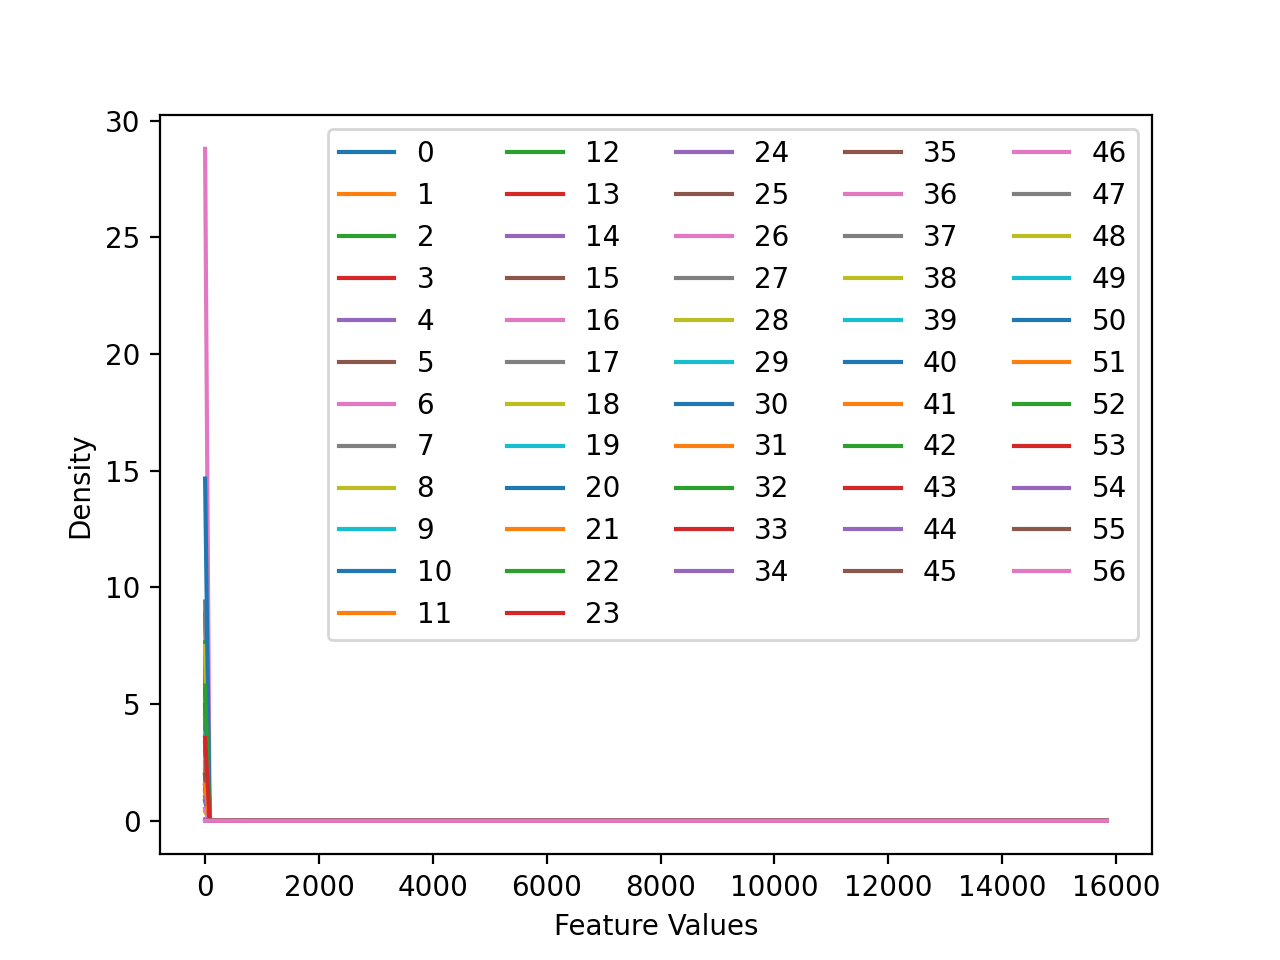
\includegraphics[width=\textwidth]{1_kde.png}
    \caption{Gaussian Kernel Density Estimation (KDE) plot.}
    \label{fig:1}
\end{figure}

\begin{figure}[H]
    \centering
    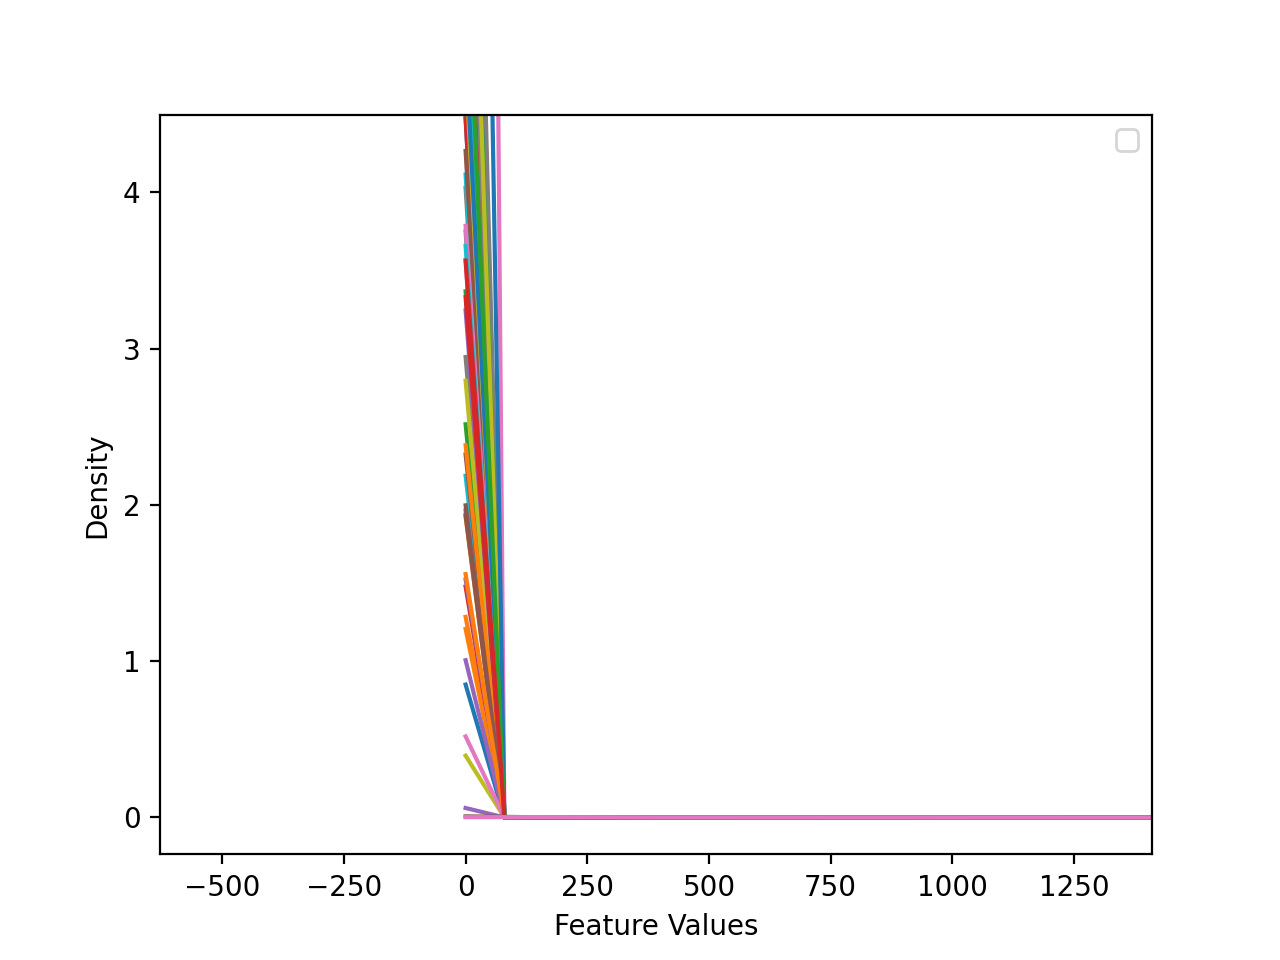
\includegraphics[width=\textwidth]{2_kde_zoommed.png}
    \caption{Zoomed in Gaussian KDE plot.}
    \label{fig:2}
\end{figure}

\begin{figure}[H]
    \centering
    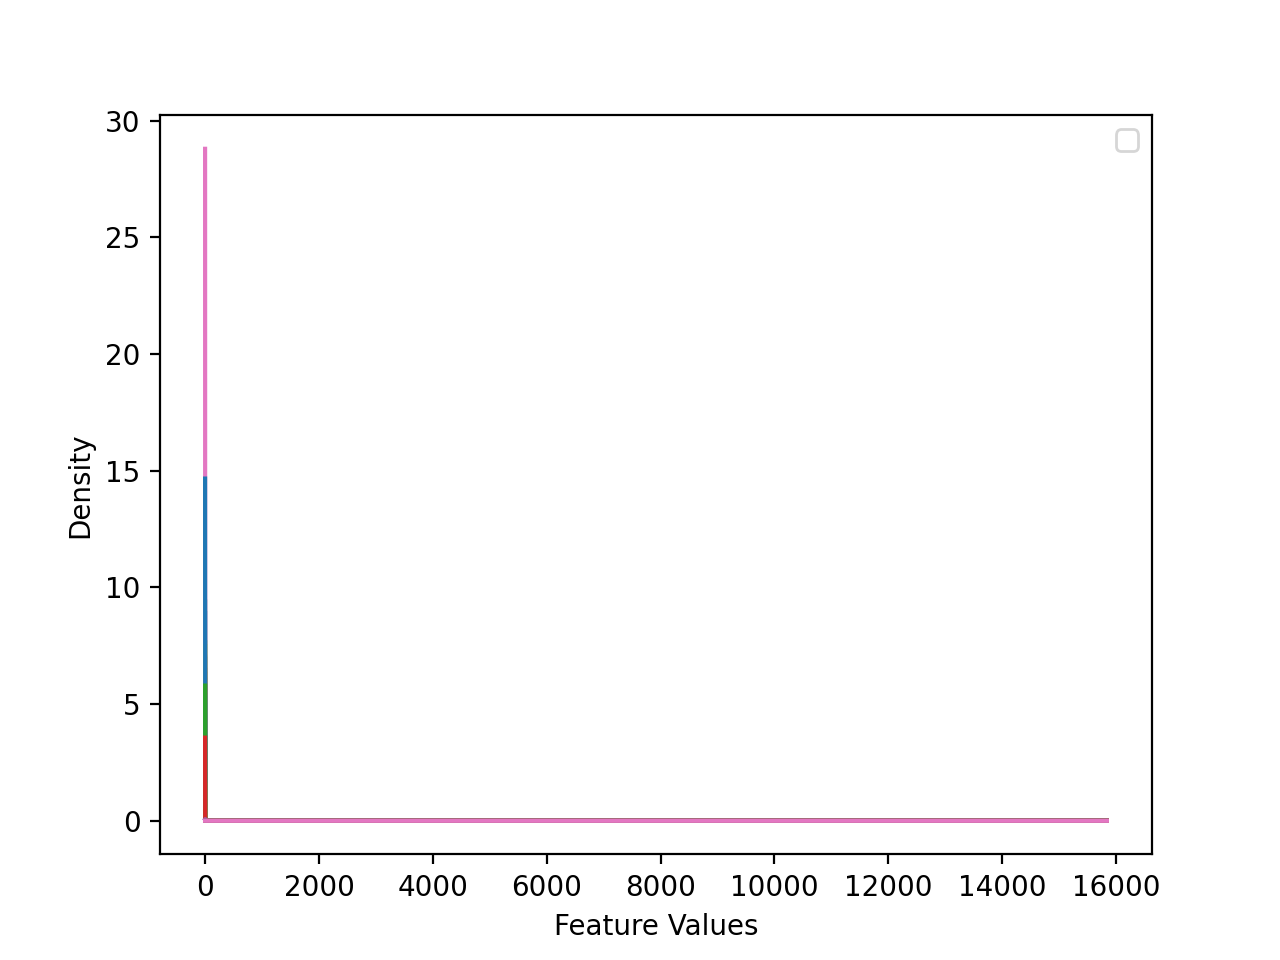
\includegraphics[width=\textwidth]{3_kde_inN.png}
    \caption{Gaussian KDE plot in more detailed stepsize.}
    \label{fig:3}
\end{figure}

\begin{figure}[H]
    \centering
    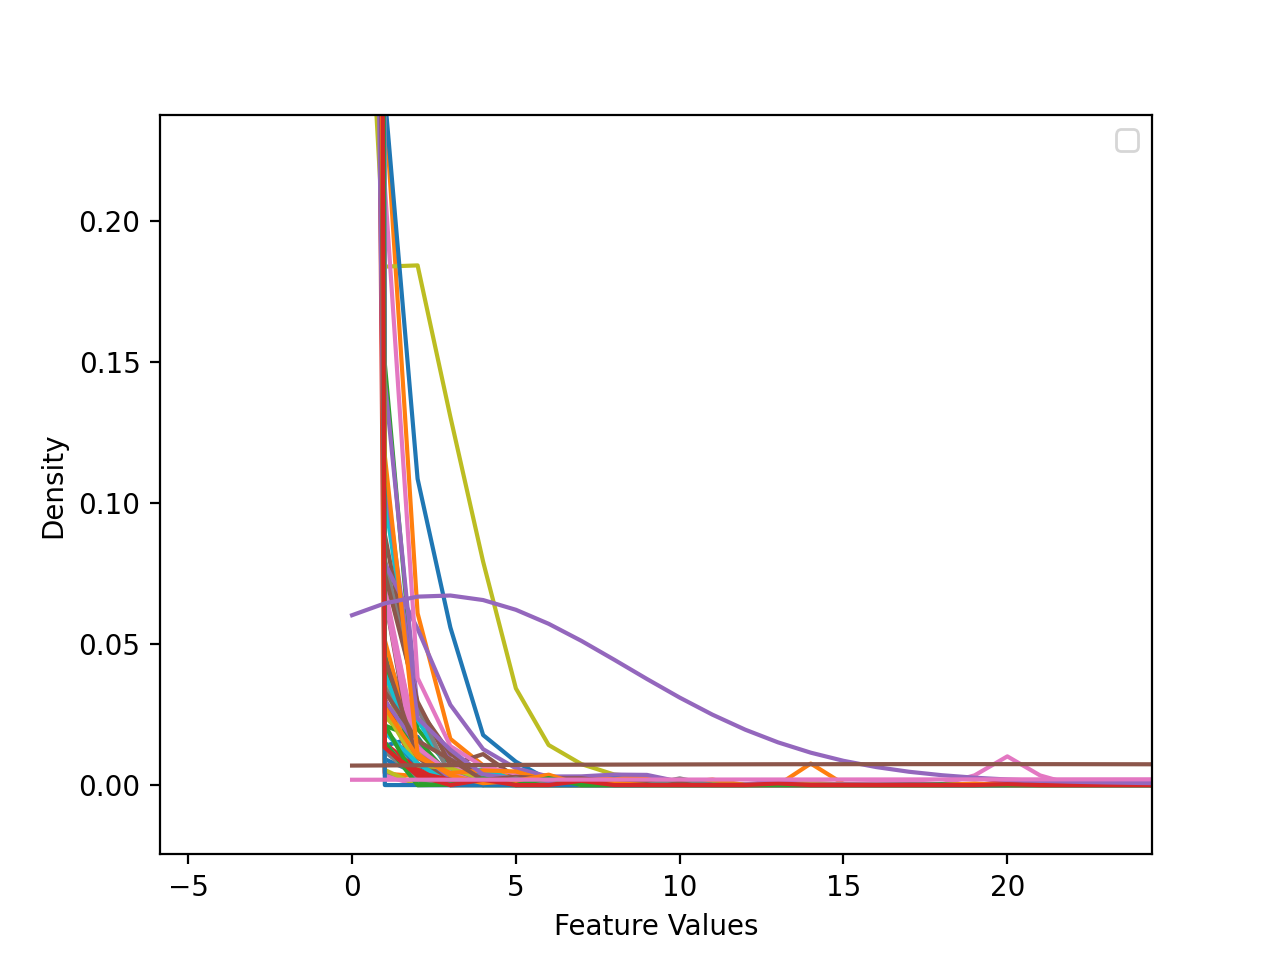
\includegraphics[width=\textwidth]{4_kde_inN_zoomed.png}
    \caption{Zoomed in Gaussian KDE plot in more detailed stepsize.}
    \label{fig:4}
\end{figure}

\begin{figure}[H]
    \centering
    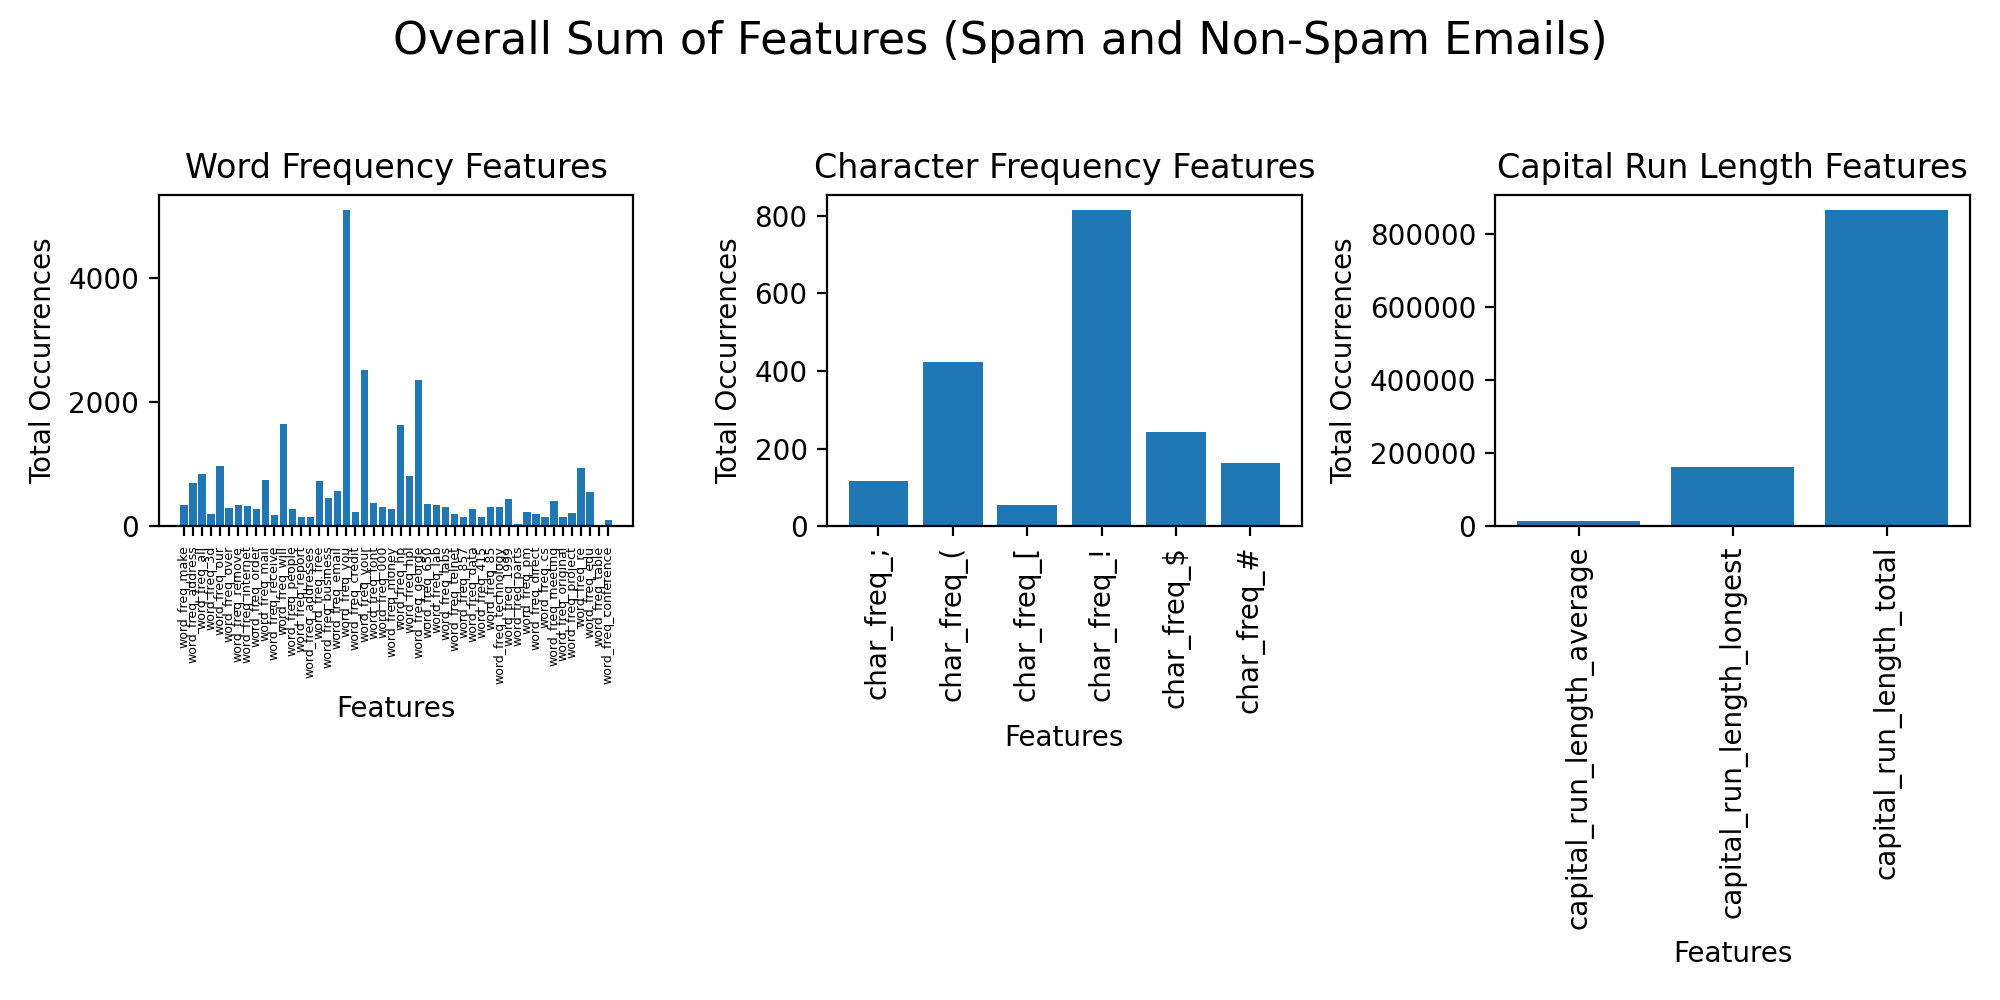
\includegraphics[width=\textwidth]{5_overall_histogram.png}
    \caption{Overall sum of feature occurency plotted in histogram.}
    \label{fig:5}
\end{figure}

\begin{figure}[H]
    \centering
    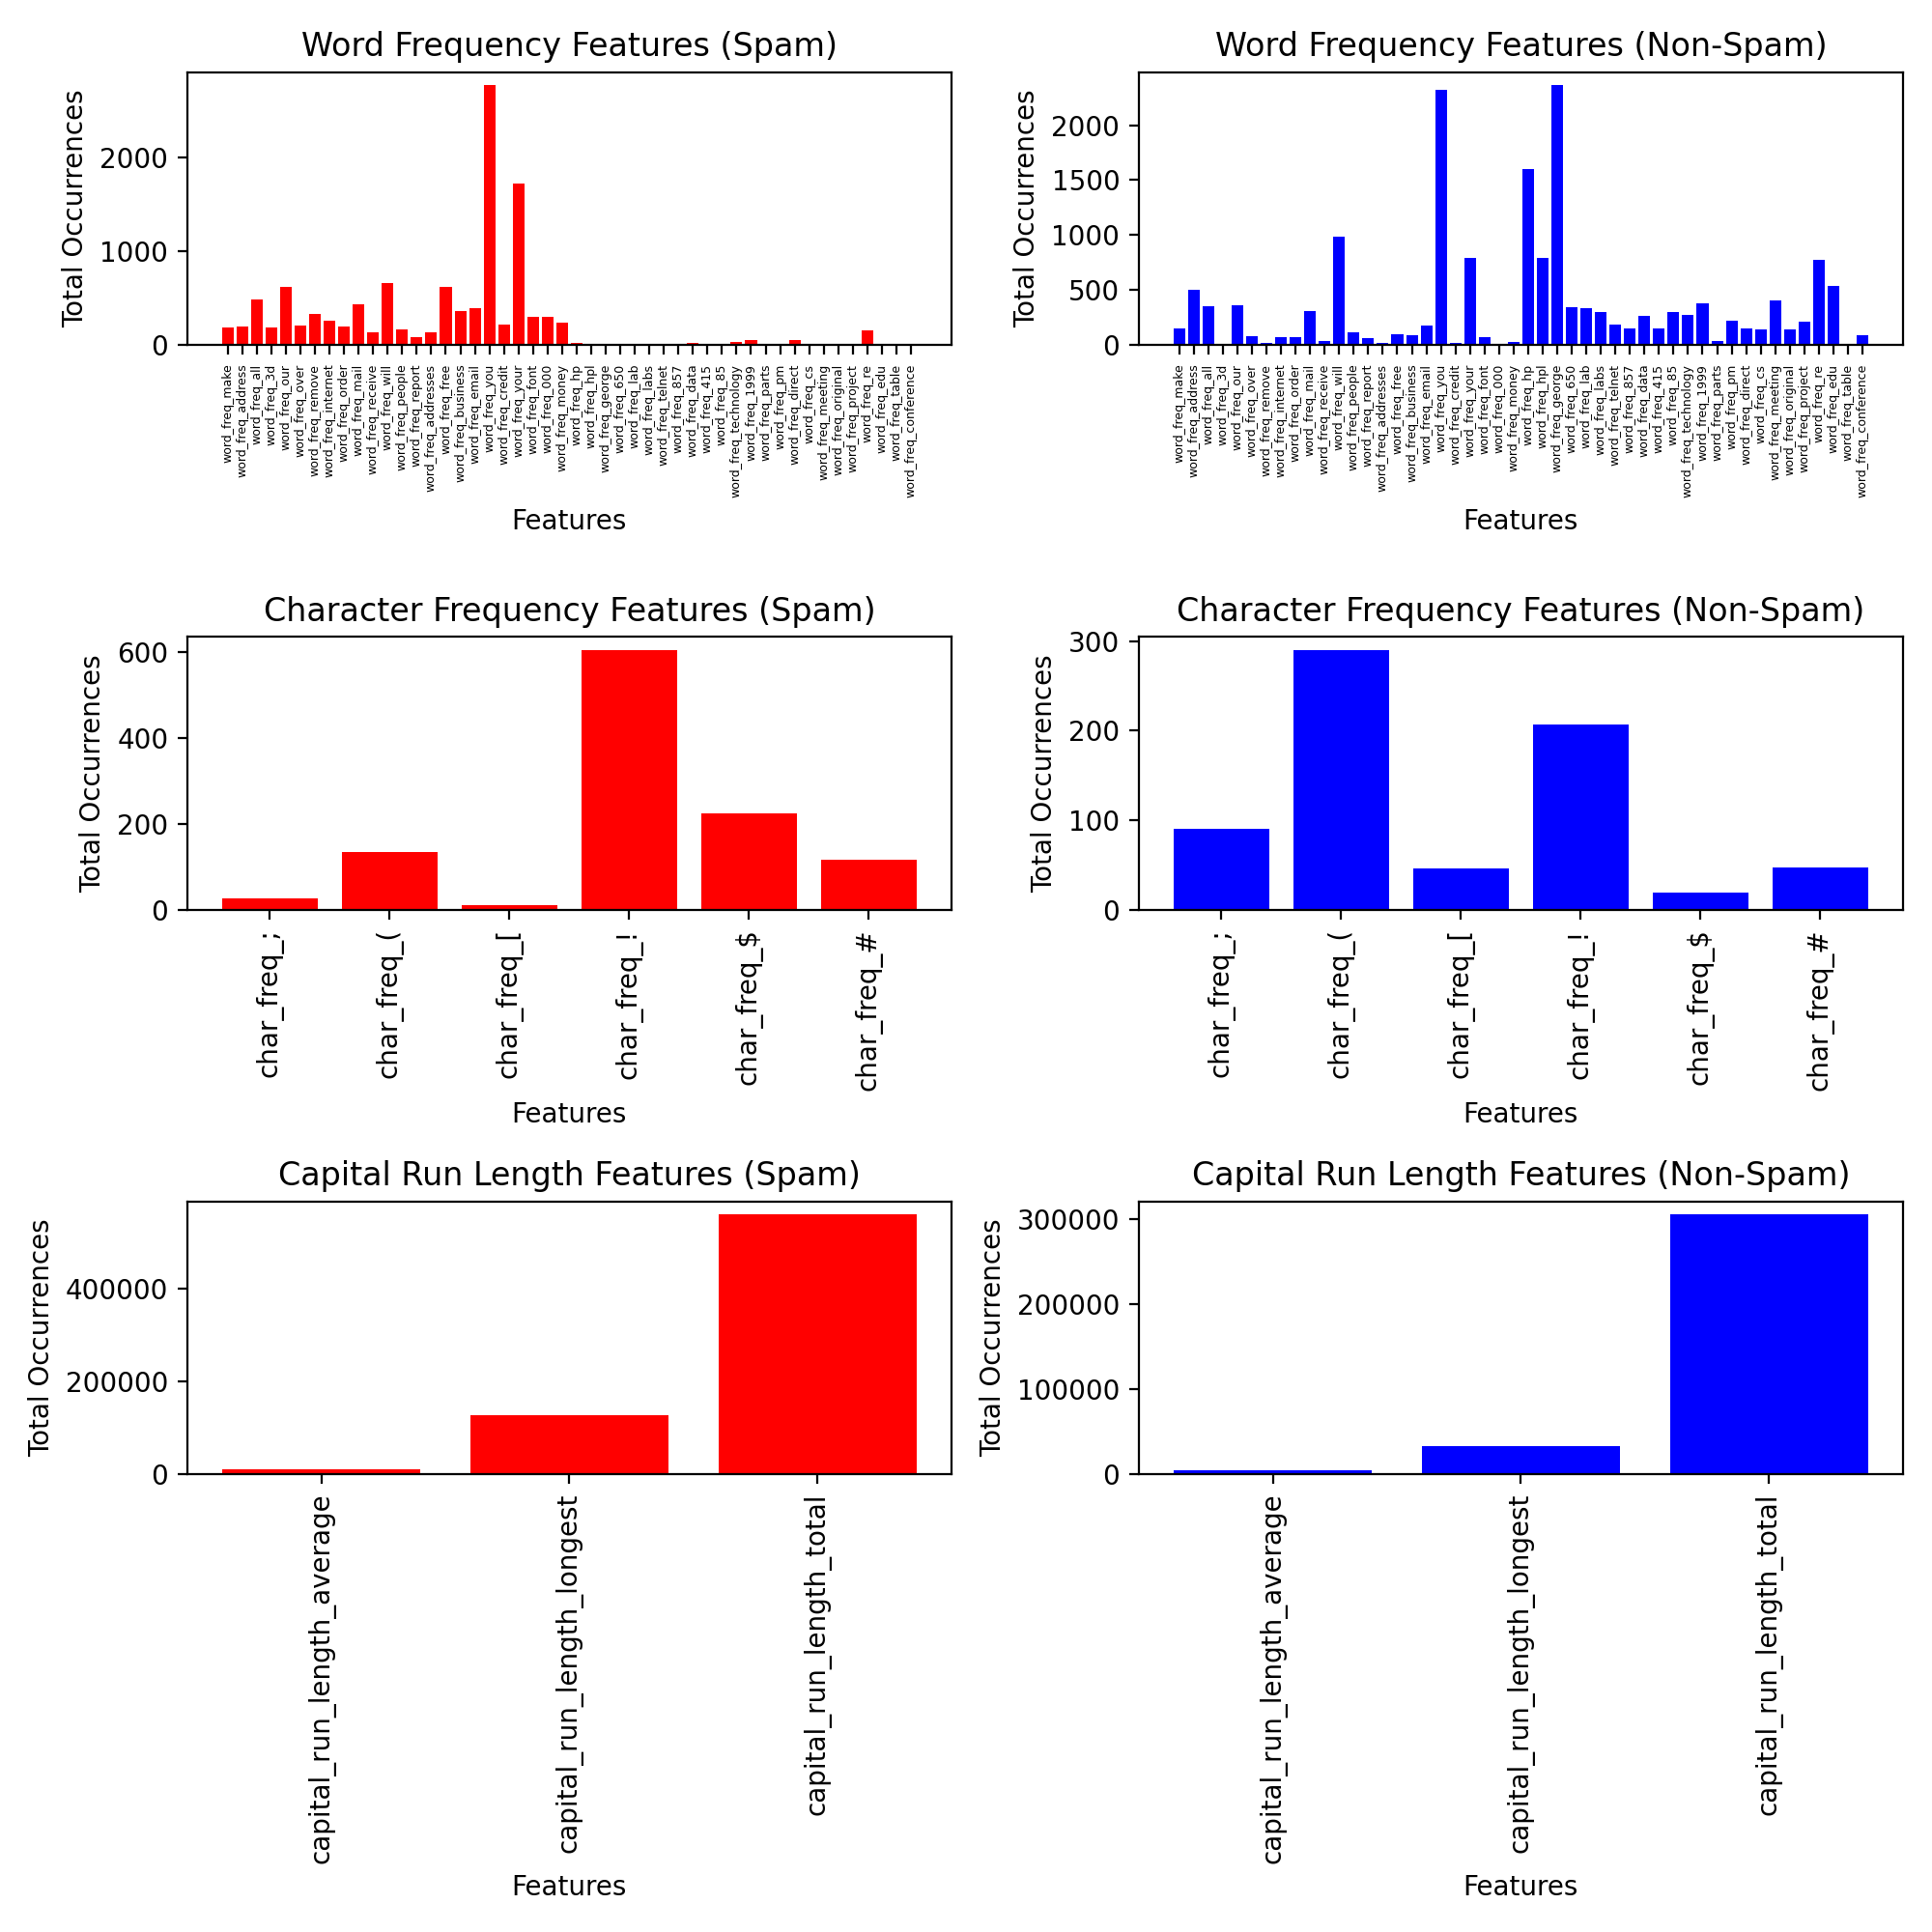
\includegraphics[width=\textwidth]{6_spam_histogram.png}
    \caption{Sum of feature occurency plotted in histogram including all spam and including all non-spam features separately.}
    \label{fig:6}
\end{figure}

\begin{figure}[H]
    \centering
    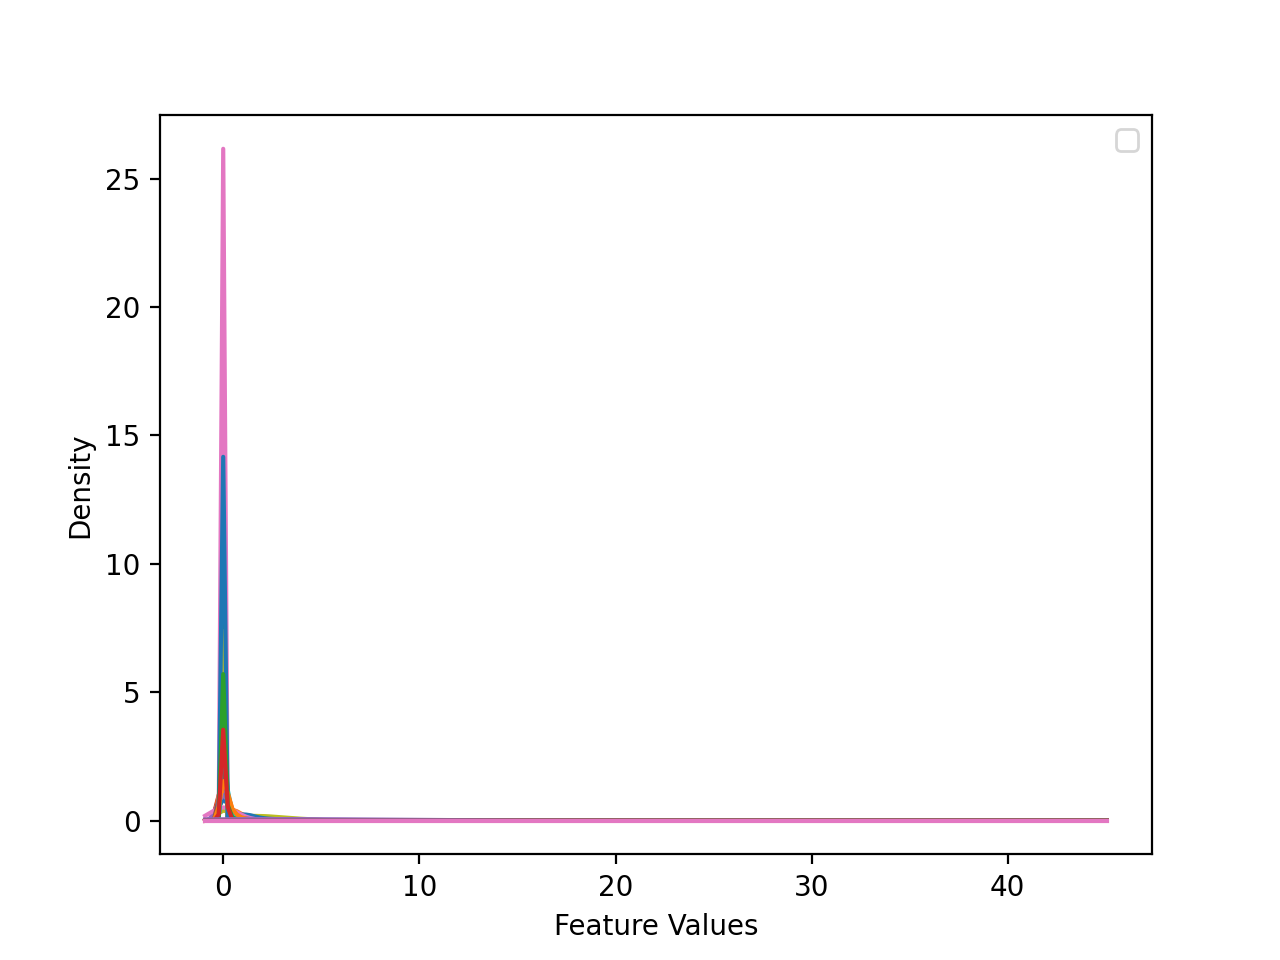
\includegraphics[width=\textwidth]{7_kde_normalized.png}
    \caption{Gaussian KDE plot with normalized data.}
    \label{fig:7}
\end{figure}

\begin{figure}[H]
    \centering
    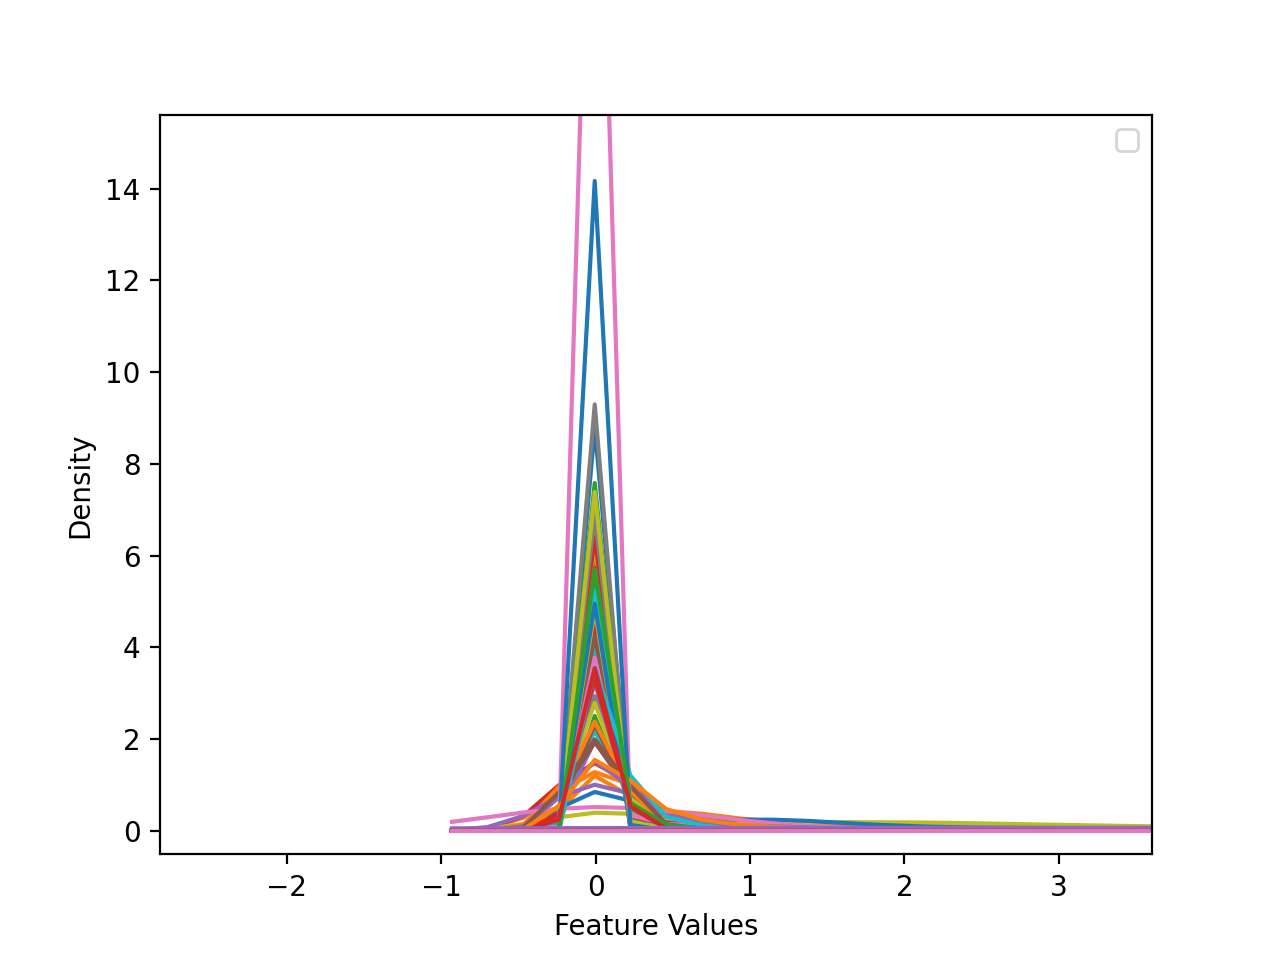
\includegraphics[width=\textwidth]{8_kde_normalized_zoomed.png}
    \caption{Zoomed in Gaussian KDE plot with normalized data.}
    \label{fig:8}
\end{figure}

\begin{figure}[H]
    \centering
    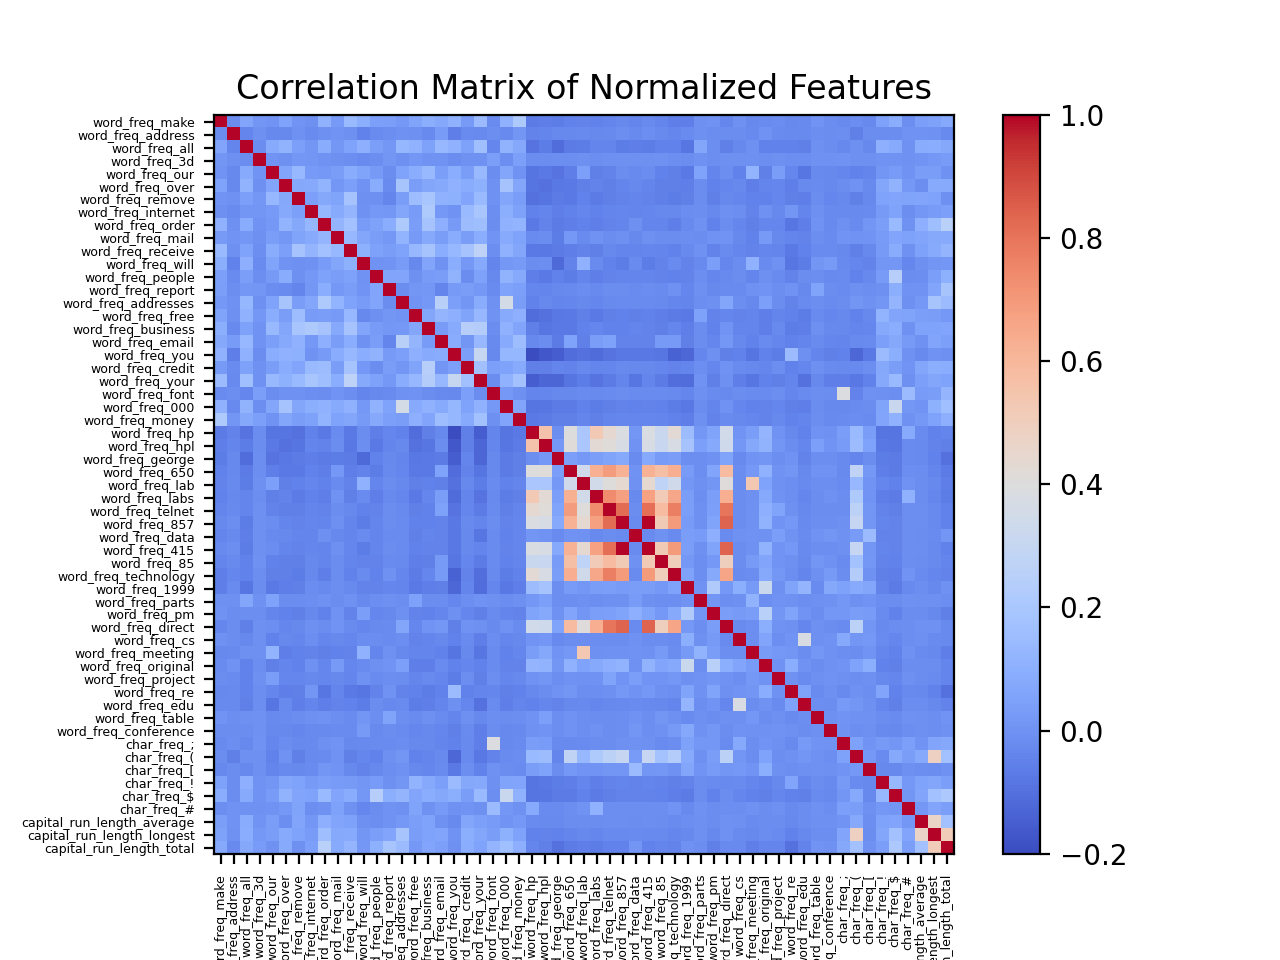
\includegraphics[width=\textwidth]{9_corrmatrix.png}
    \caption{Correlation matrix of normalized features.}
    \label{fig:9}
\end{figure}


\section{Plots and Outputs for Task 2}
\label{section2}

\begin{figure}[H]
    \centering
    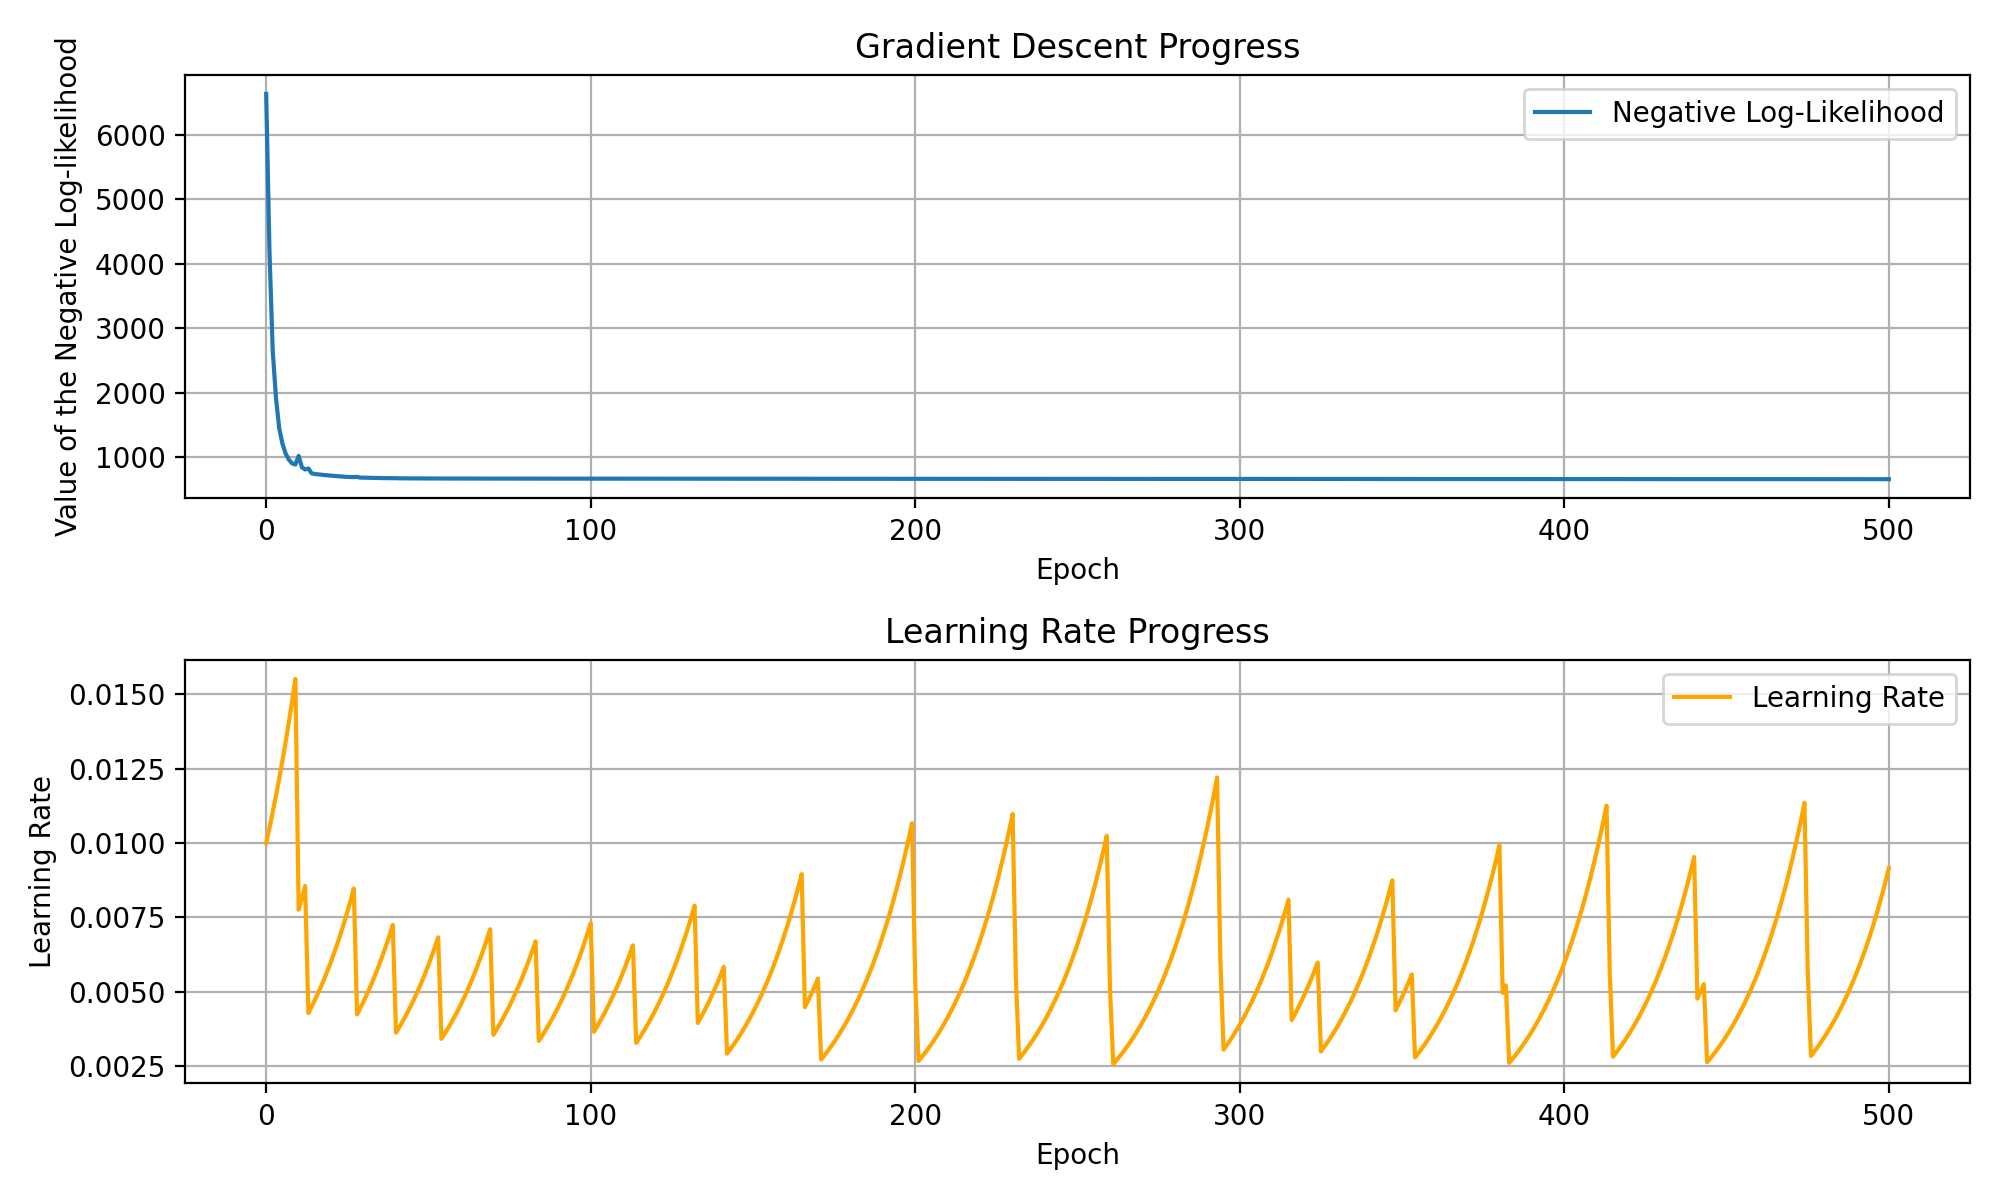
\includegraphics[width=\textwidth]{10_GD progress.png}
    \caption{Gradient Descent progress visualized in the progress of the negative log-likelihood and the learning rate over the epochs.}
    \label{fig:10}
\end{figure}

\begin{figure}[H]
    \centering
    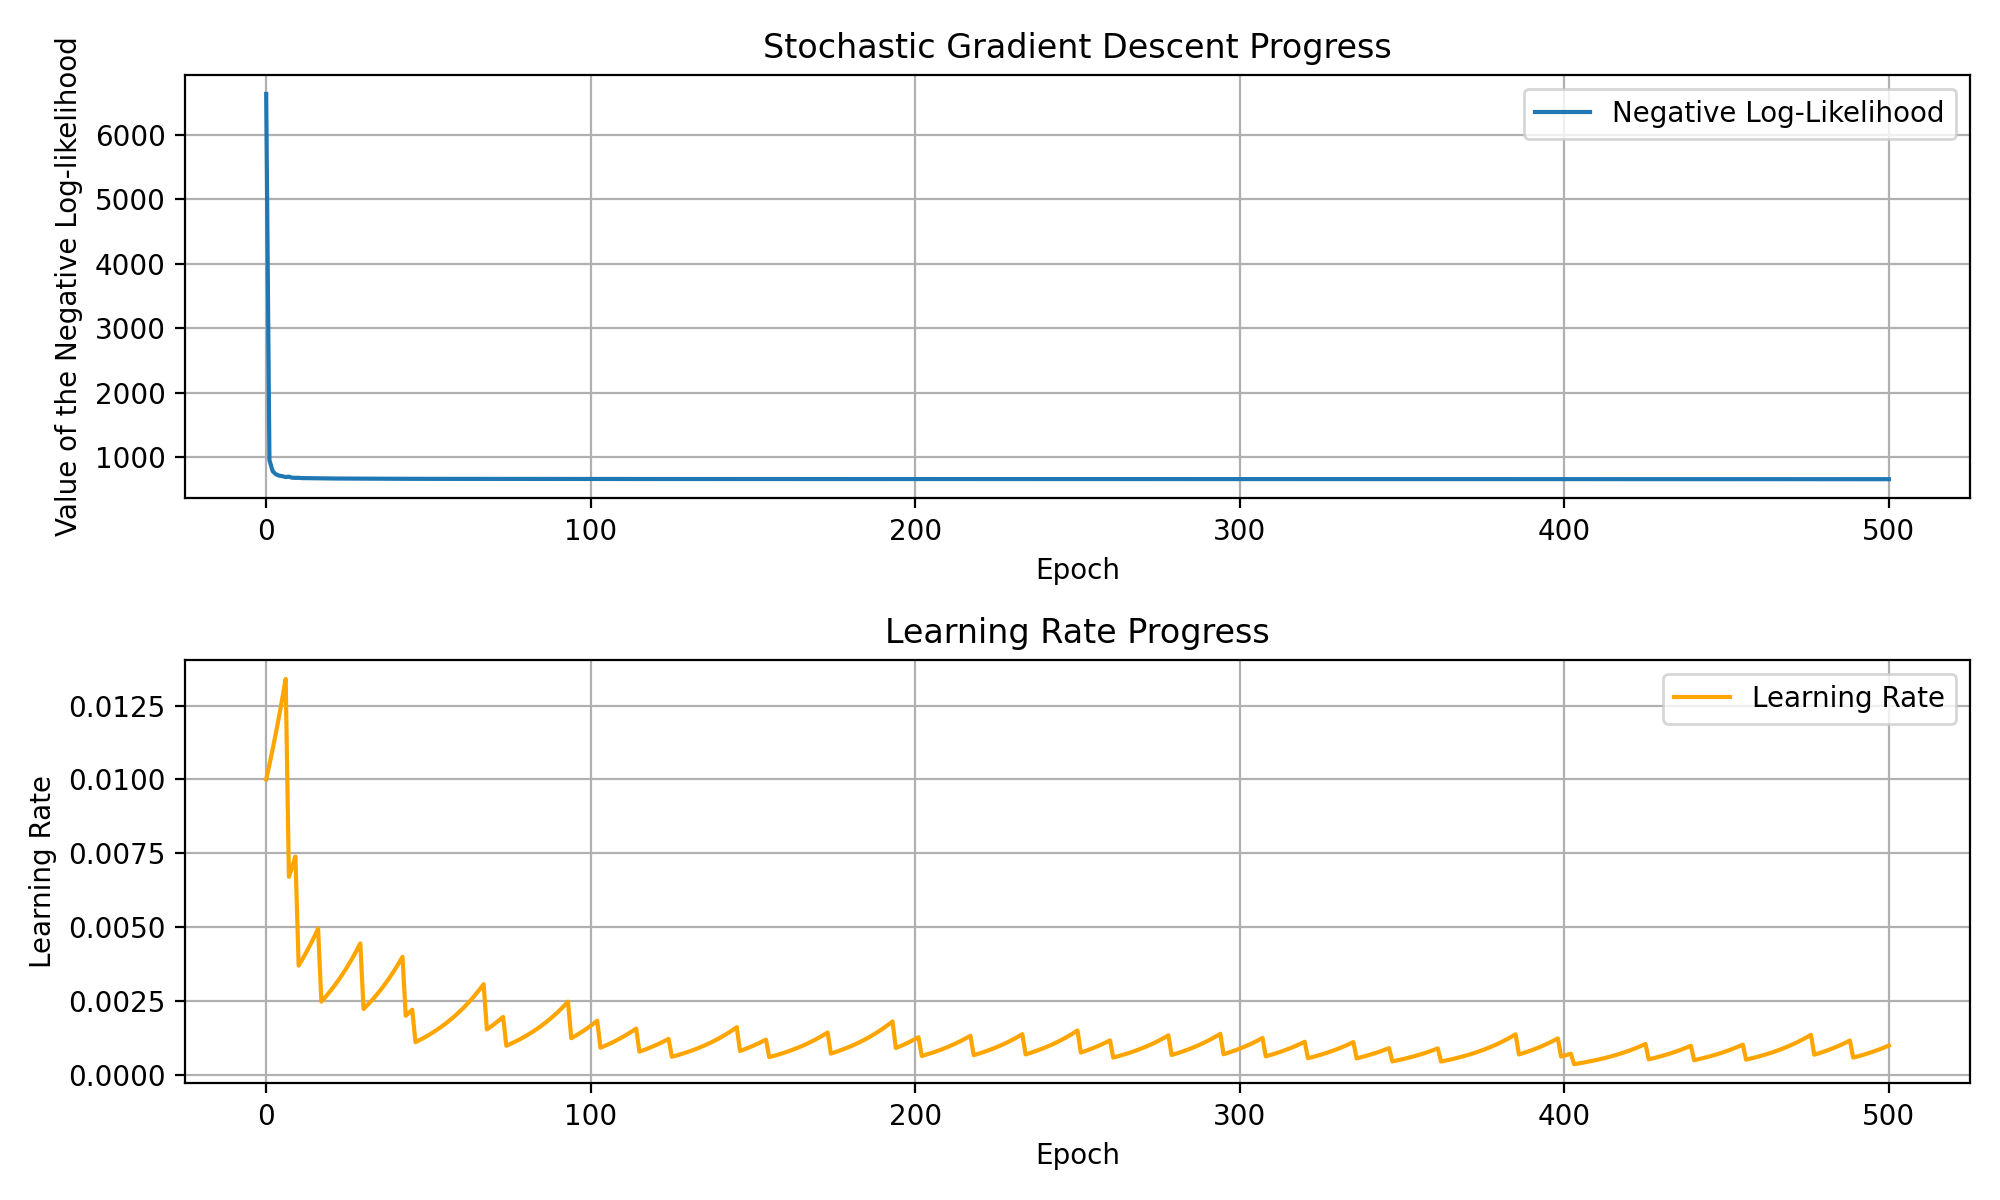
\includegraphics[width=\textwidth]{11_sgd progress.png}
    \caption{Stochastic Gradient Descent progress visualized in the progress of the negative log-likelihood and the learning rate over the epochs.}
    \label{fig:11}
\end{figure}

\begin{figure}[H]
    \centering
    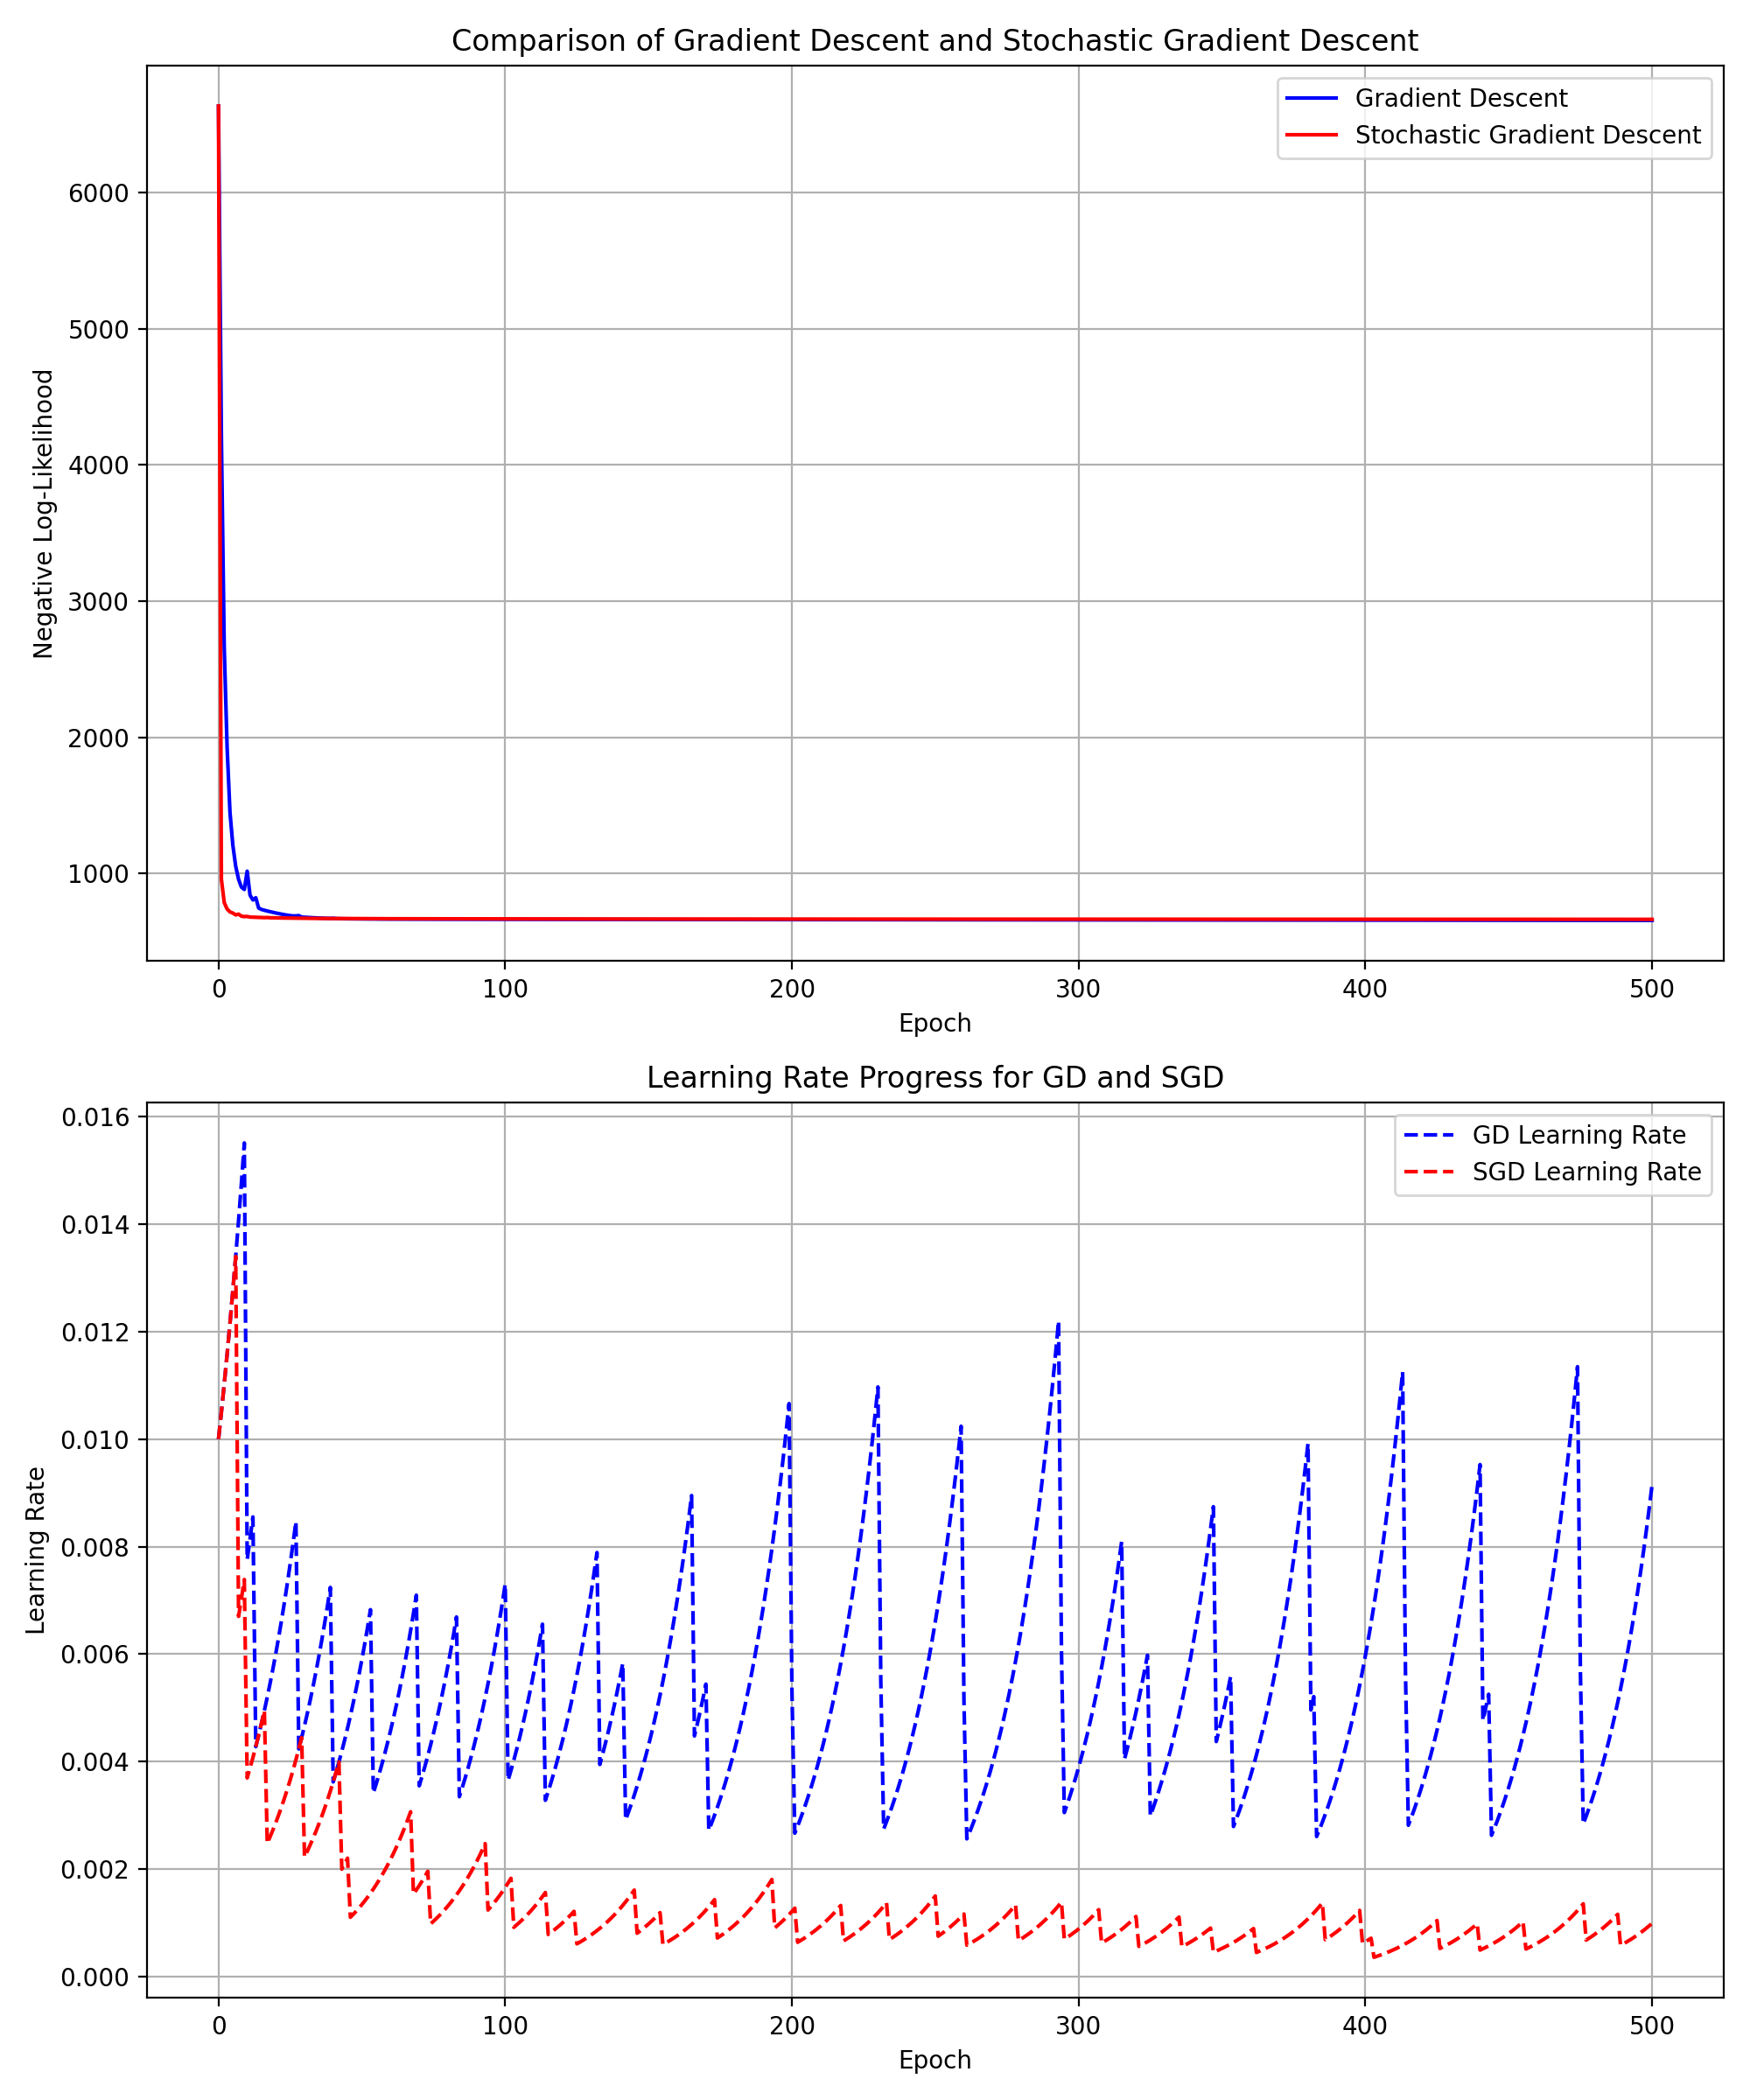
\includegraphics[width=\textwidth]{12_gd and sgd comparison.png}
    \caption{Comparison of GD and SGD via the progress of the negative log-likelihood and the learning rate.}
    \label{fig:12}
\end{figure}

\section{Outputs and Plot for Task 3}
\label{section3}


\subsection{Confusion Matrix and Model Comparison}
The confusion matrices for both Gradient Descent (GD) and Stochastic Gradient Descent (SGD) models provide insight into the classification outcomes for the test set (\texttt{ytest}) using normalized input data (\texttt{Xtestz}). In comparing the results:

\begin{itemize}
    \item \textbf{True Positives (TP):} GD identified 507 true positives, while SGD identified 508. This indicates a slight advantage for SGD in correctly classifying spam emails.
    \item \textbf{True Negatives (TN):} GD identified 876 true negatives, while SGD identified 878. This difference reflects that SGD is slightly more effective in identifying legitimate (non-spam) emails.
    \item \textbf{False Positives (FP):} GD misclassified 65 non-spam emails as spam, while SGD had 63 false positives. This suggests that GD is marginally less precise in distinguishing non-spam emails.
    \item \textbf{False Negatives (FN):} GD had 88 false negatives, while SGD had 87, indicating that SGD misses fewer spam emails.
\end{itemize}

The minor differences between GD and SGD are consistent with the models’ stochasticity and learning processes, as SGD’s stochastic updates yield slightly better performance in spam detection (higher TP, lower FN), while GD slightly reduces the misclassification of legitimate emails (higher TN, lower FP).

\subsection{Evaluation Metrics}
The following evaluation metrics, calculated for the GD model, provide insight into the model’s accuracy, precision, recall, and overall balance. Similar results were observed for the SGD model.

\begin{itemize}
    \item \textbf{Accuracy:} The accuracy for GD is calculated as
    \[
    \text{Accuracy} = \frac{TP + TN}{TP + TN + FP + FN} = \frac{507 + 876}{507 + 876 + 65 + 88} \approx 0.9004,
    \]
    indicating that approximately 90.04\% of instances were correctly classified.

    \item \textbf{Precision:} The precision for the spam class in GD is
    \[
    \text{Precision} = \frac{TP}{TP + FP} = \frac{507}{507 + 65} \approx 0.8863,
    \]
    meaning that around 88.63\% of instances predicted as spam are indeed spam.

    \item \textbf{Recall:} Recall, indicating the percentage of actual spam instances correctly identified, is
    \[
    \text{Recall} = \frac{TP}{TP + FN} = \frac{507}{507 + 88} \approx 0.8521.
    \]

    \item \textbf{F1 Score:} The F1 score for GD is the harmonic mean of precision and recall:
    \[
    \text{F1 Score} = 2 \times \frac{\text{Precision} \times \text{Recall}}{\text{Precision} + \text{Recall}} \approx 0.8690.
    \]
\end{itemize}


\begin{figure}[H]
    \centering
    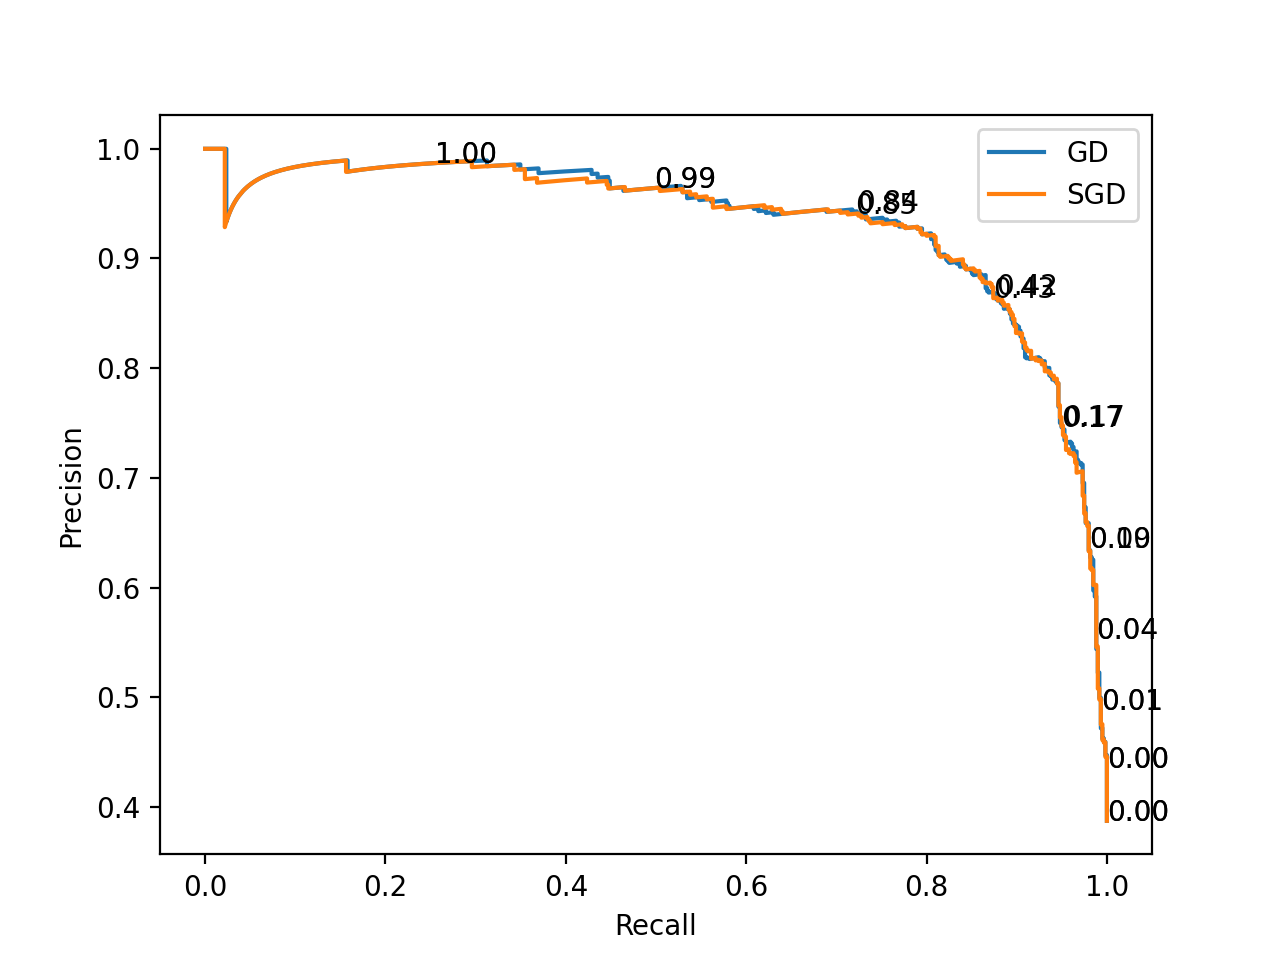
\includegraphics[width=\textwidth]{13_precision_recall_curve.png}
    \caption{Precision-Recall curve plotted for GD and SGD.}
    \label{fig:13}
\end{figure}

\section{Plots and Outputs for Task 4}
\label{section4}

\begin{figure}[H]
    \centering
    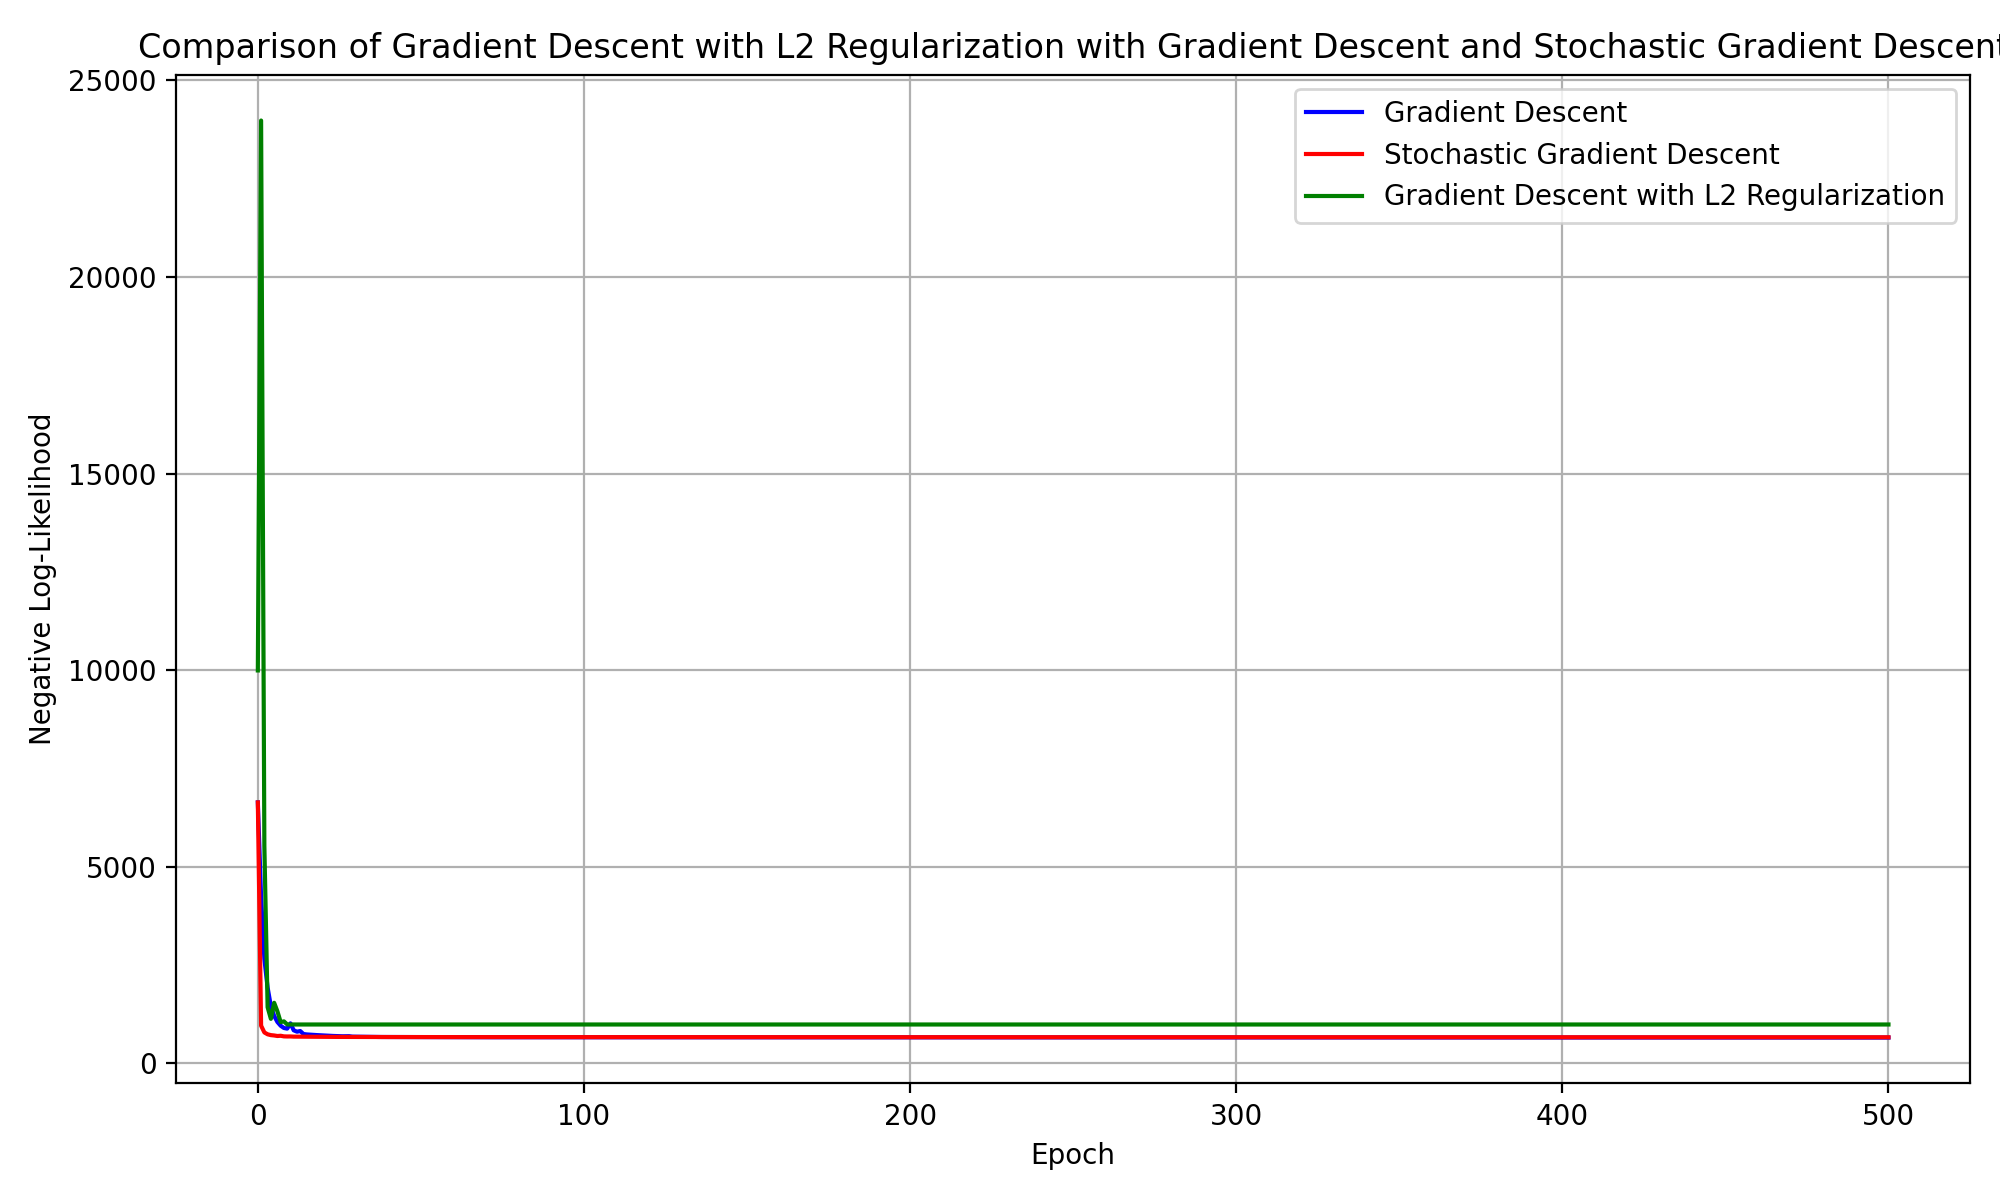
\includegraphics[width=\textwidth]{14_gd_l2 comparison.png}
    \caption{Comparison of GD with L2 regularization with GD and SGD in the progress of the negative log-likelihood.}
    \label{fig:14}
\end{figure}

\begin{figure}[H]
    \centering
    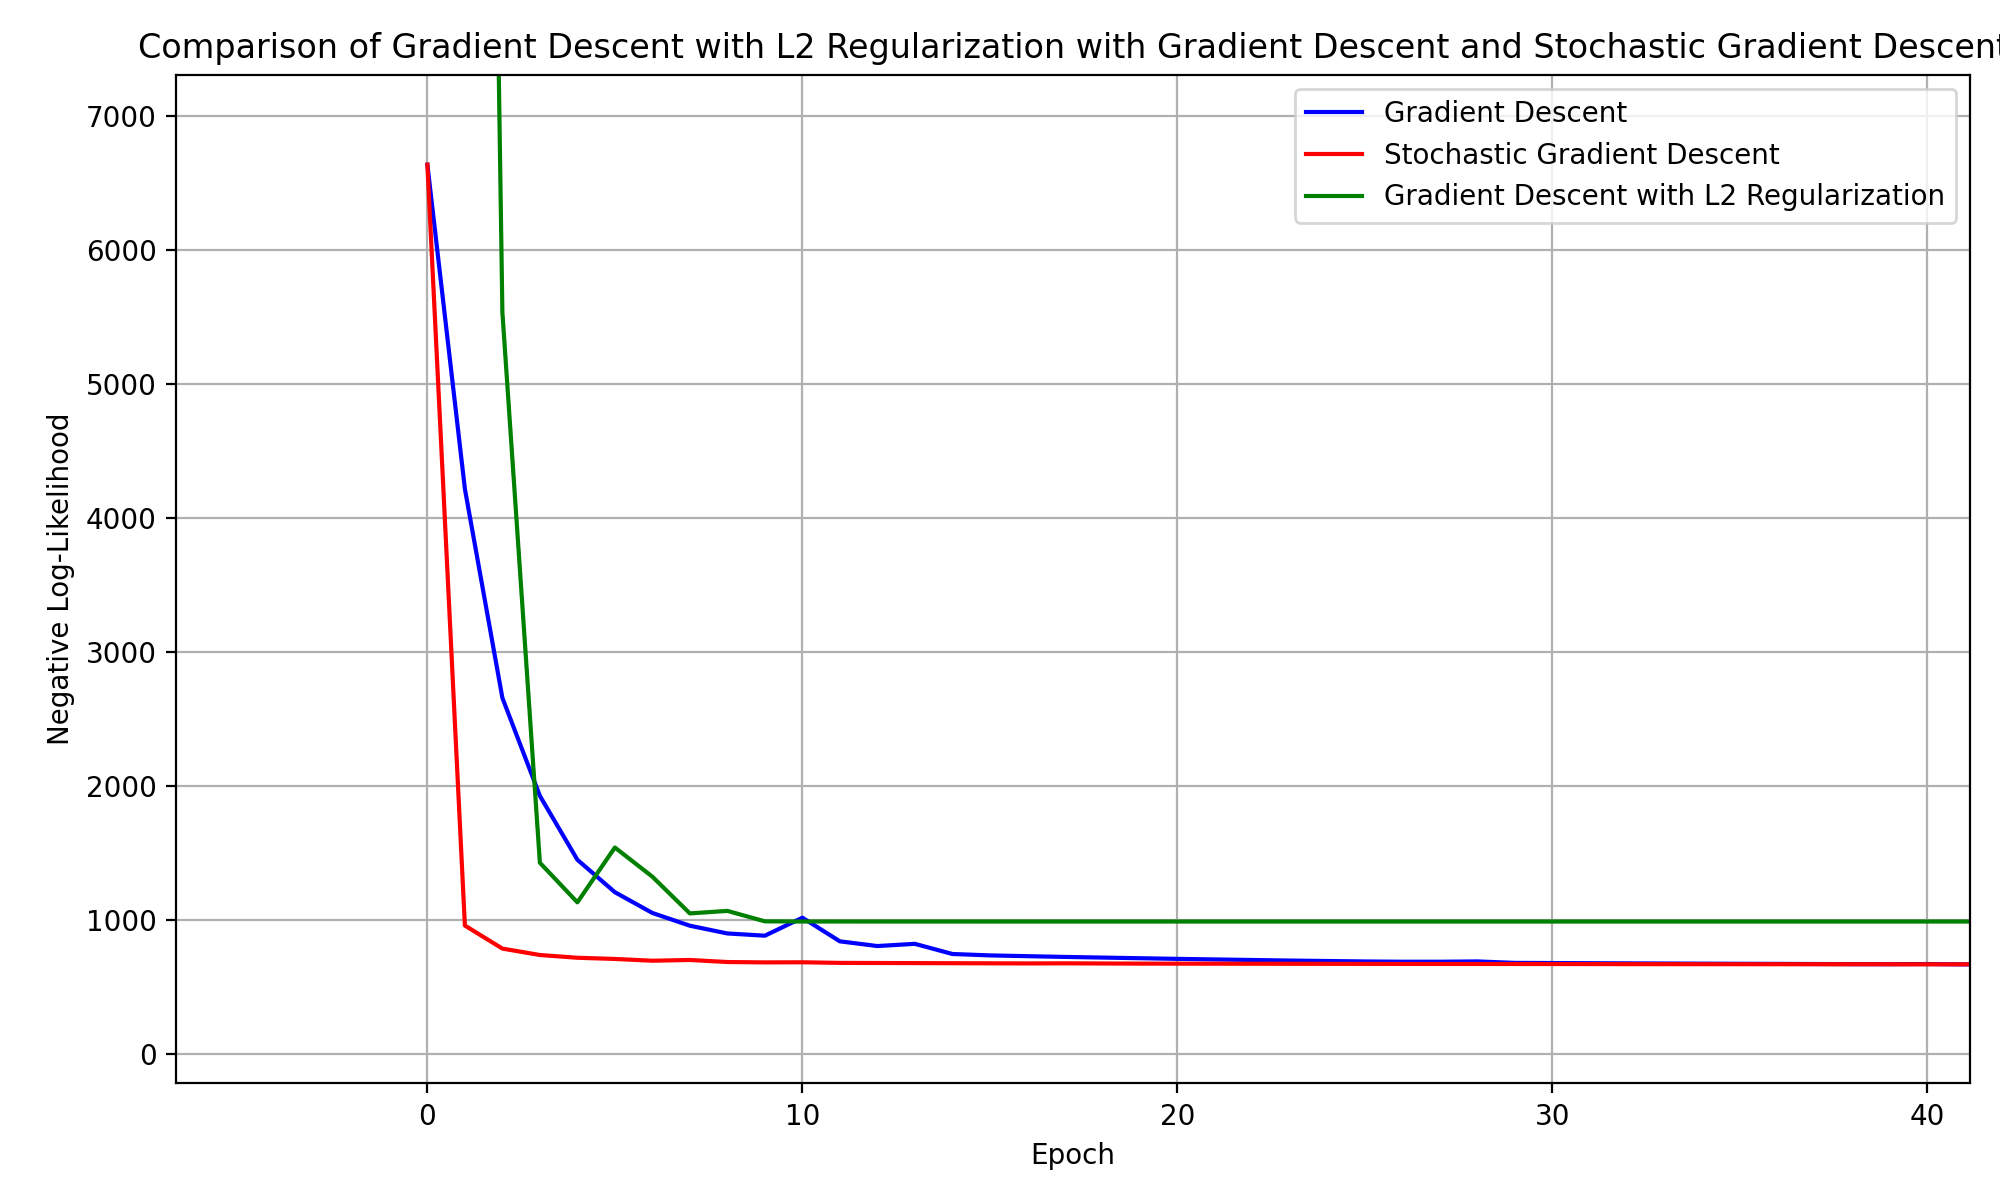
\includegraphics[width=\textwidth]{15_gd_l2 comparison zoomed.png}
    \caption{Zoomed in comparison of GD with L2 regularization with GD and SGD in the progress of the negative log-likelihood.}
    \label{fig:15}
\end{figure}

\begin{figure}[H]
    \centering
    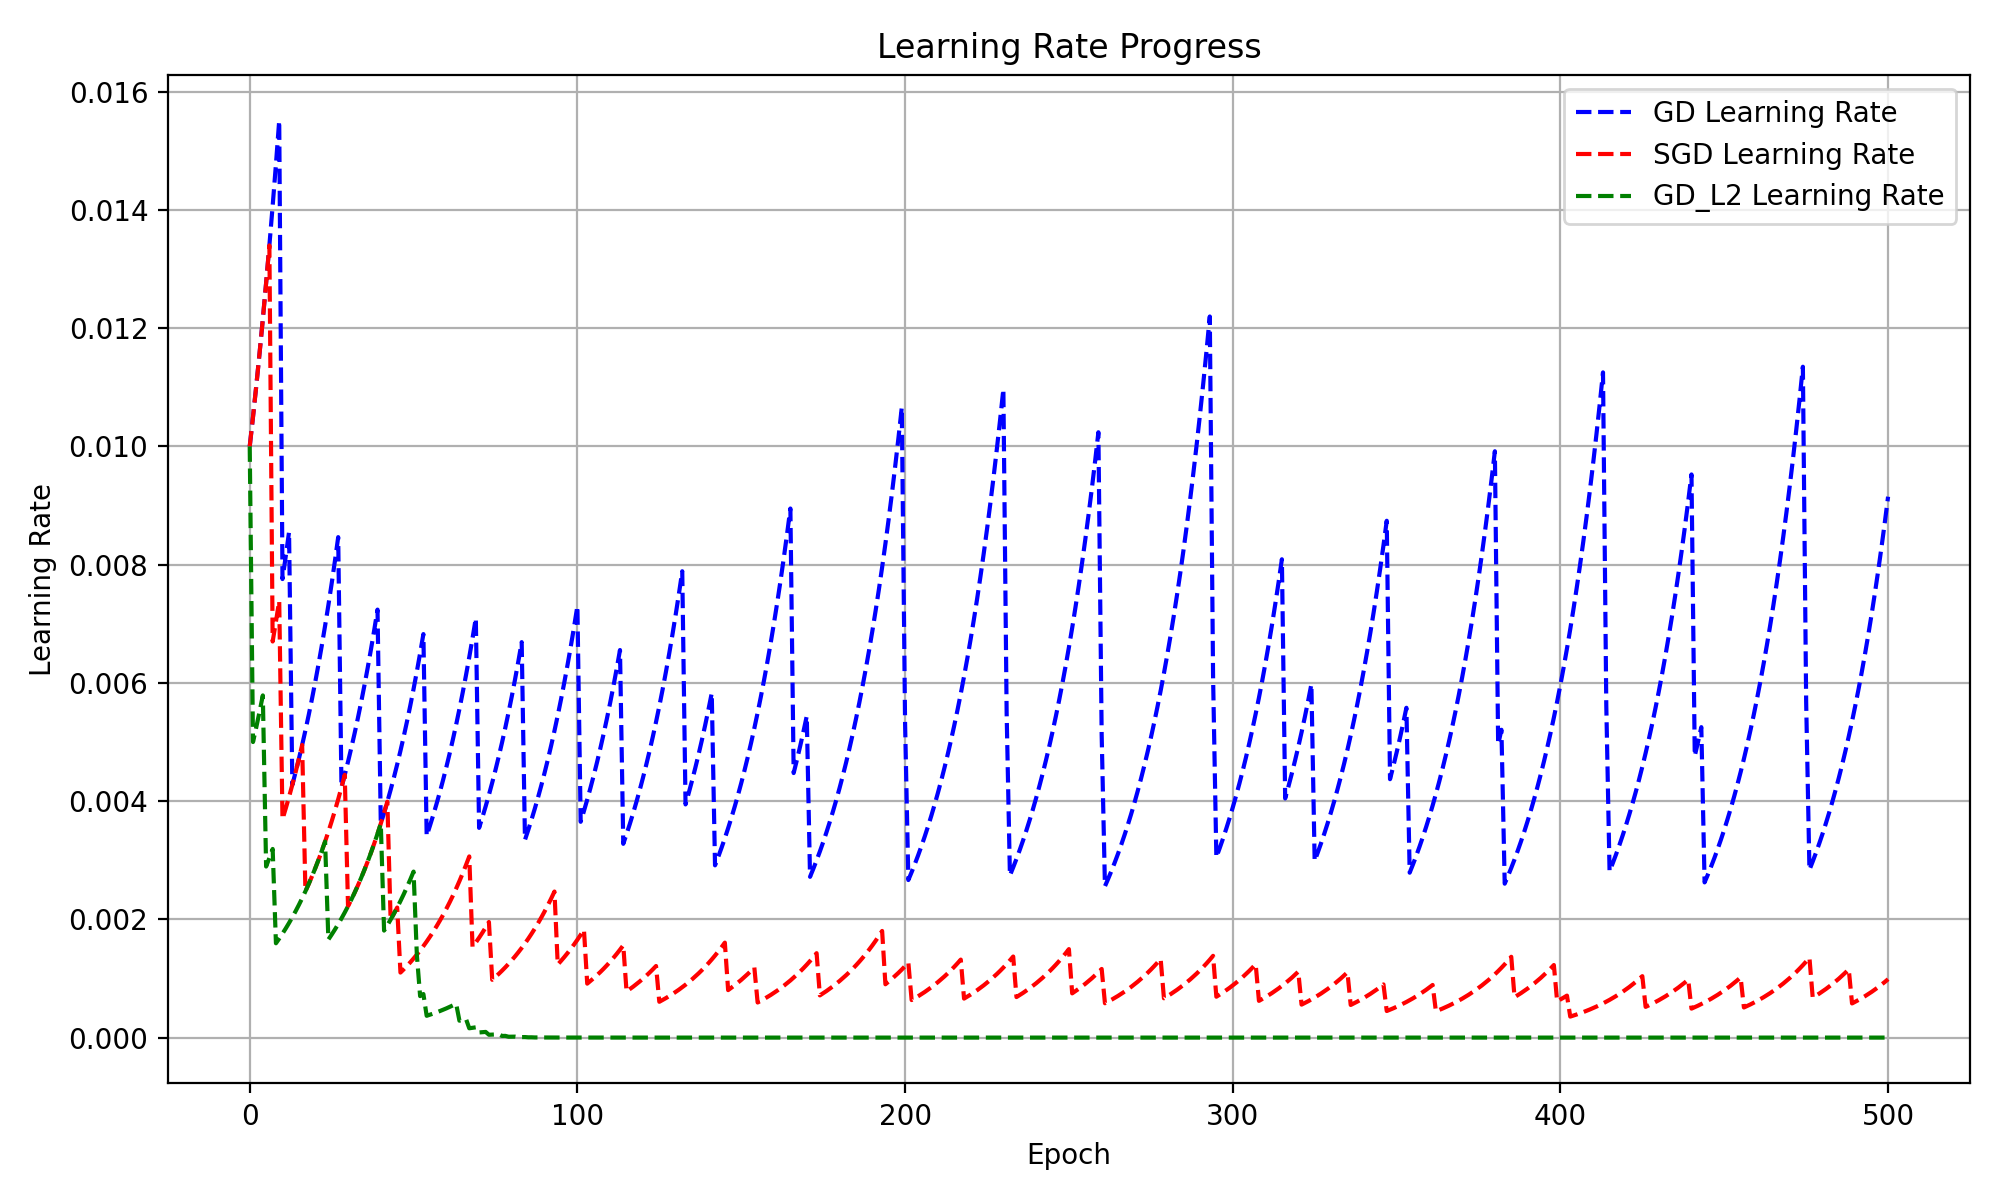
\includegraphics[width=\textwidth]{16_gd_l2 learning rate.png}
    \caption{Comparison of GD with L2 regularization with GD and SGD in the progress of the learning rate.}
    \label{fig:16}
\end{figure}


\subsection{Precision, Recall, and F1 Score Analysis}
\label{section4p}

Precision, recall, and F1 score follow similar trends to accuracy, as shown in Figure \ref{fig:17}. At lower $\lambda$ values, these metrics remain stable, indicating balanced performance in both positive and negative classes. As $\lambda$ approaches values around 1 to 10, precision, recall, and F1 scores reach their highest values, reflecting an optimal regularization effect that avoids overfitting while capturing key patterns in the data. For larger $\lambda$ values, these scores decrease markedly, emphasizing that excessive regularization reduces the model’s ability to identify positive class instances effectively. Thus, moderate values of $\lambda$ yield the best balance across these classification metrics, while extreme values degrade performance by imposing strong constraints on parameter values.

\subsection{AUC Score and $\lambda$ Sensitivity}

The AUC score exhibits a smaller range of variation compared to other metrics, as shown in Figure \ref{fig:17}. Starting from an initial value of approximately 0.958, AUC slightly increases with moderate $\lambda$ values and reaches a peak near 0.959, indicating improved classification boundary separation. However, as $\lambda$ grows further, AUC declines to around 0.952, reflecting a decrease in ranking quality when the model becomes overly regularized. The relatively stable AUC values across varying $\lambda$ indicate that ranking quality remains robust even as accuracy and other metrics fluctuate more significantly.

\subsection{Summary of Findings}

The analysis demonstrates that $\lambda$ plays a crucial role in determining the model’s performance. A balanced $\lambda$ value, in the range of 1 to 10, enables the model to achieve high classification accuracy and effective generalization without excessive overfitting. At very high values, the L2 penalty restricts the model’s flexibility, leading to significant underfitting and a drop in all performance metrics except for a comparatively less affected AUC score.

In conclusion, the results underscore that an optimal $\lambda$ balances error minimization and generalization. While low $\lambda$ values permit better fit on the training data, they risk overfitting, as indicated by disparities between training and test log-likelihoods. Moderate $\lambda$ values effectively reduce overfitting while retaining the model’s flexibility, as evidenced by improvements in log-likelihoods, accuracy, and F1 score. Excessive $\lambda$ values, however, impose excessive constraints, limiting the model’s ability to capture essential data patterns. These findings, illustrated in Figures \ref{fig:14} through \ref{fig:17}, confirm that the choice of $\lambda$ is essential to achieving a model that generalizes well without compromising predictive accuracy.



\begin{figure}[H]
    \centering
    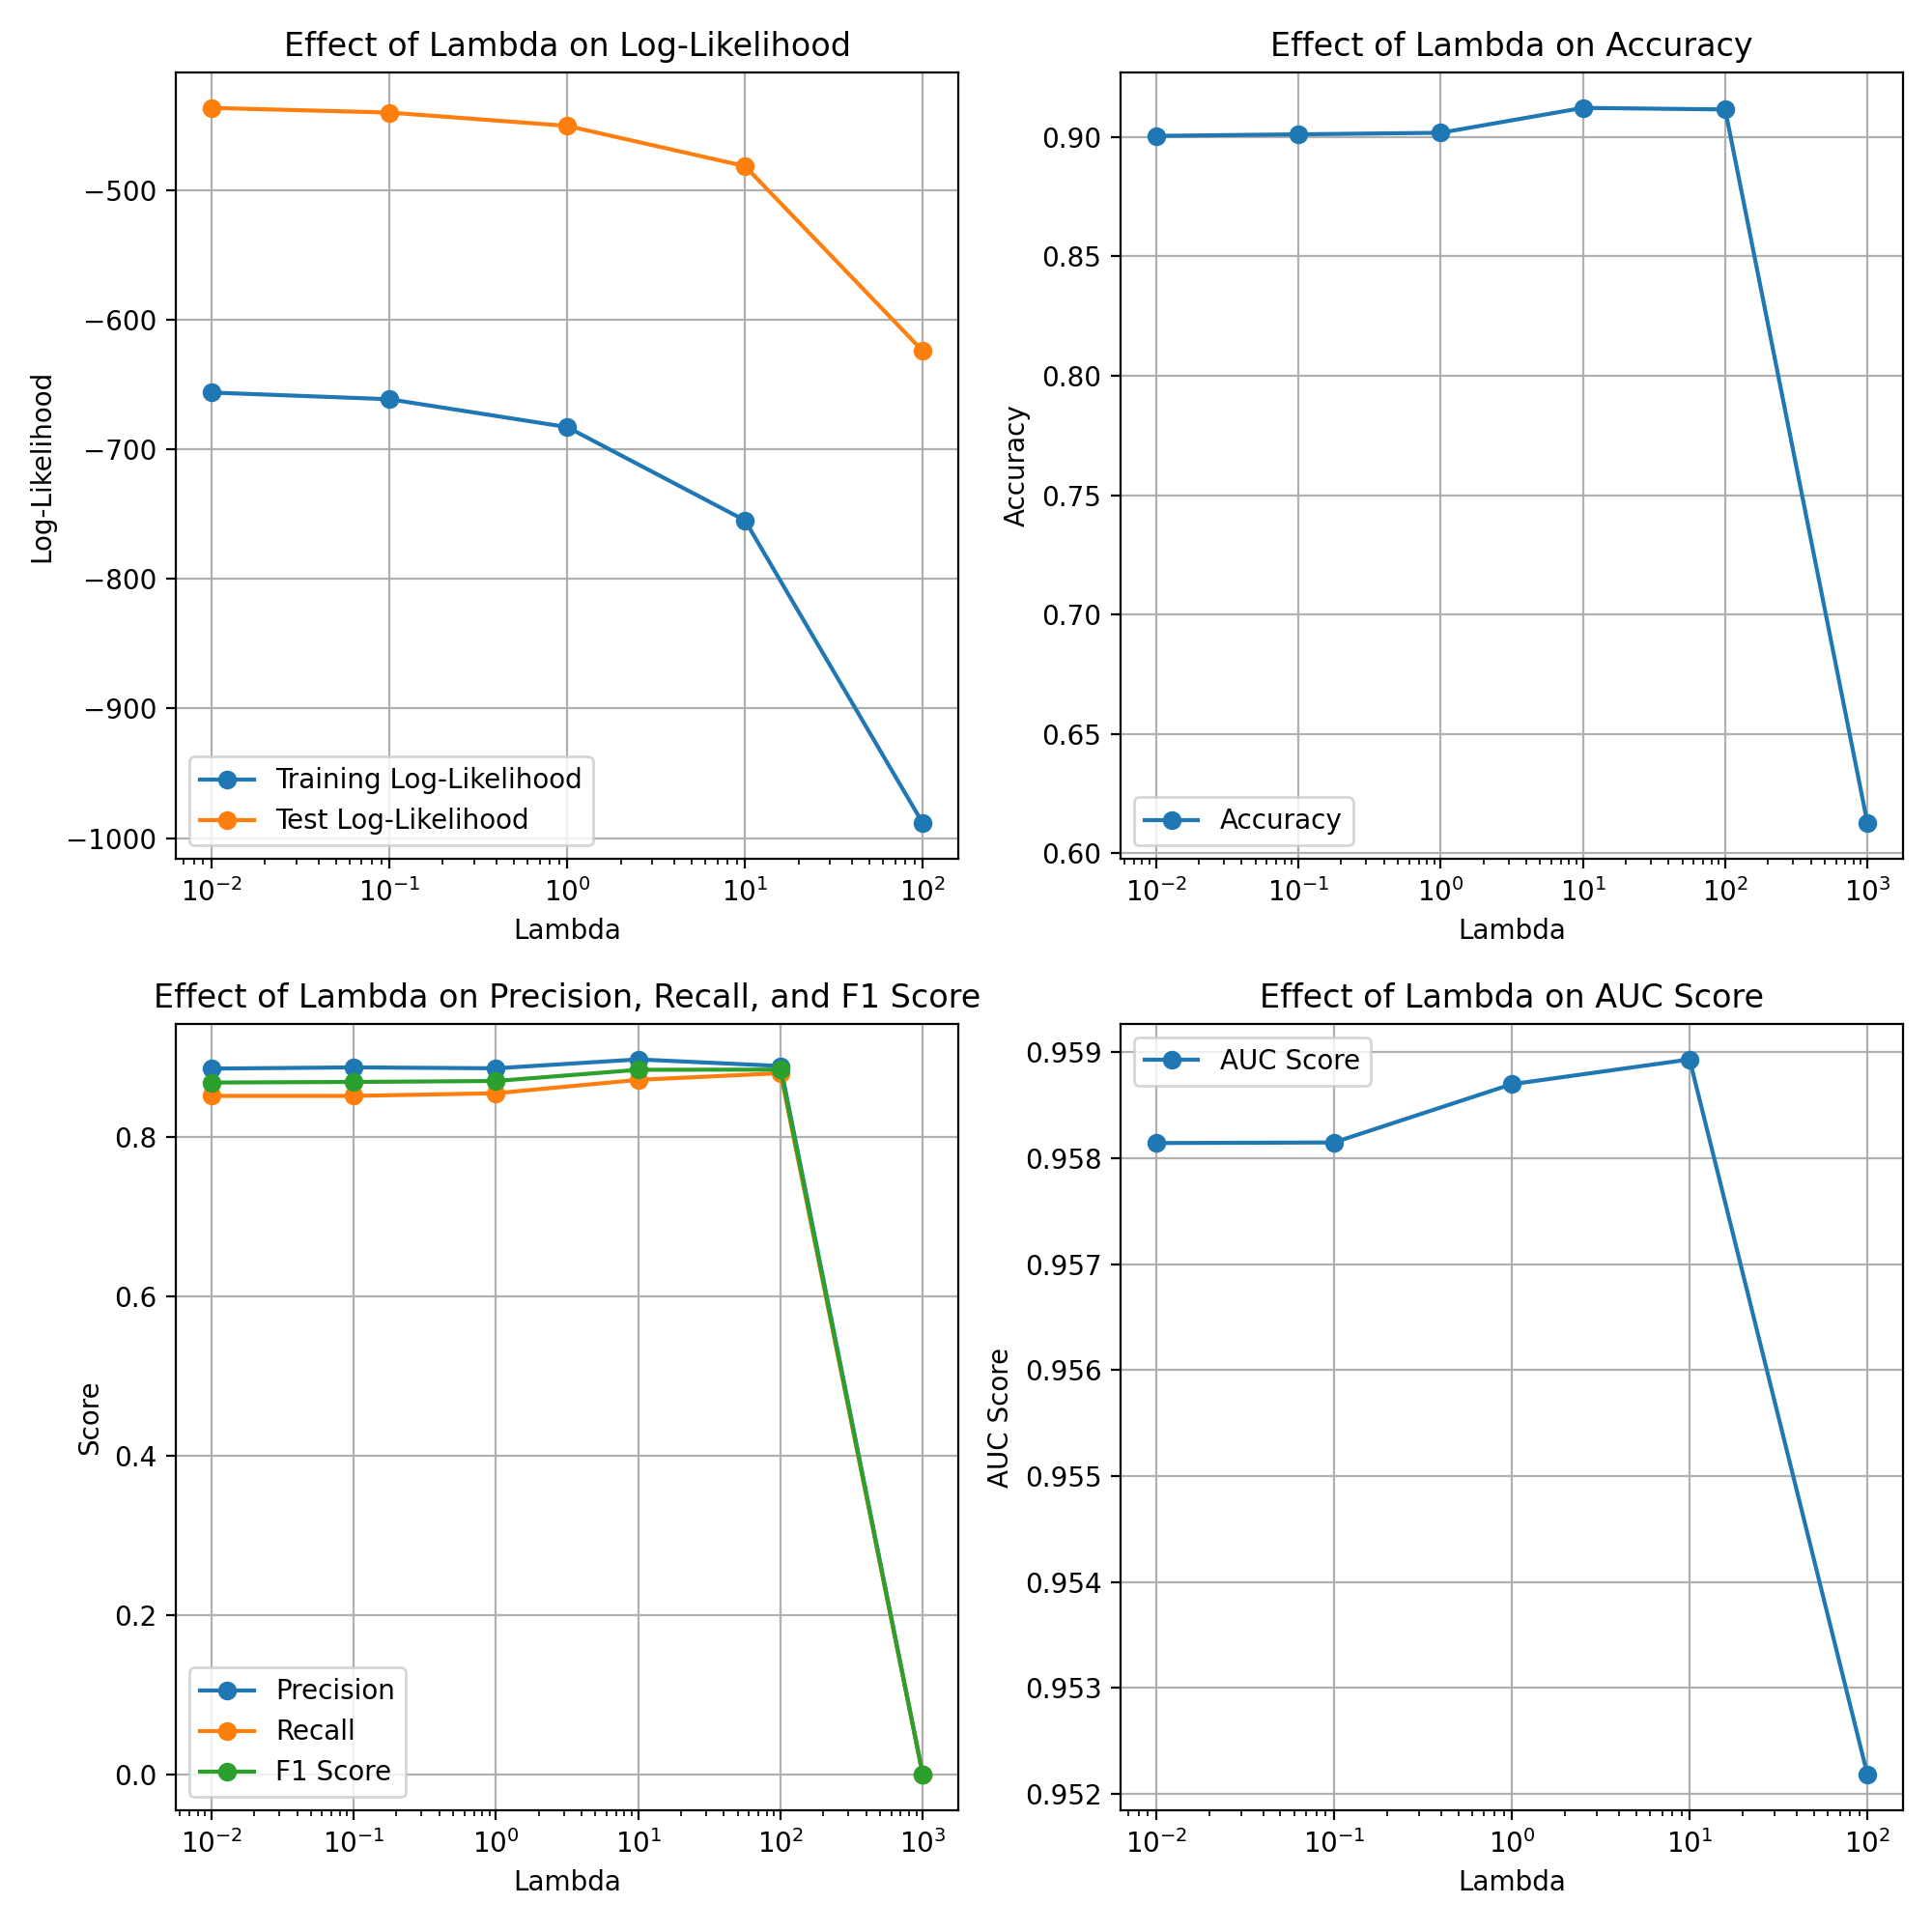
\includegraphics[width=\textwidth]{17_lambda.png}
    \caption{Effect of different Lambda parameter size.}
    \label{fig:17}
\end{figure}
 

\clearpage
\section*{Declaration of Honor}

I hereby declare that I have written the enclosed 
project report without the help of third parties and without the use of other
sources and aids other than those listed in the table below
and that I have identified the passages taken from the sources used verbatim or in terms of content as such.
or content taken from the sources used. This work has not been submitted in the same or a similar form
been submitted to any examination authority. I am aware that a false declaration
declaration will have legal consequences.

% Declare below which AI tools you used in the process of writing your work,
% including text, image, code, and data generation. If you used a tool for a
% purpose not included in the list yet, add it to the list.
\begin{center}
  \textbf{Declaration of Used AI Tools} \\[.3em]
  \begin{tabularx}{\textwidth}{lXlc}
    \toprule
    Tool & Purpose & Where? & Useful? \\
    \midrule
    ChatGPT & Rephrasing & Throughout & + \\
    DeepL & Translation & Throughout & + \\
    %ResearchGPT & Summarization of related work & Sec.~\ref{sec:related_work} & - \\
    %Dall-E & Image generation & Figs.~2, 3 & ++ \\
    Github Copilot & Code generation & a02-lr.ipynb & + \\
    %ChatGPT & Related work hallucination & Most of bibliography & ++ \\
    \bottomrule
  \end{tabularx}
\end{center}

\vspace{2cm}
\noindent Signatures\\
\noindent Mannheim, 03. November 2024 \hfill

\end{document}